\documentclass[11pt]{article}
\usepackage[utf8]{inputenc}
\usepackage[dvips]{graphicx}
\usepackage{graphicx}
\usepackage{fancybox}
\usepackage{verbatim}
\usepackage{array}
\usepackage{latexsym}
\usepackage{alltt}
\usepackage{hyperref}
\usepackage{textcomp}
\usepackage{color}
\usepackage{amsmath}
\usepackage{amsfonts}
\usepackage{tikz}
\usepackage{float}
\usepackage{pdfpages}
\usepackage[most]{tcolorbox}
\usepackage[hmargin=3cm,vmargin=5.0cm]{geometry}
\usepackage{centernot}
\usepackage[table,xcdraw]{xcolor}
\usepackage{wrapfig}
\usepackage{subfigure}
\usepackage{minted}
\usepackage{listings}
\usepackage{algorithm}
\usepackage[noend]{algpseudocode}
%\topmargin=0cm
\topmargin=-2cm
\addtolength{\textheight}{6.5cm}
\addtolength{\textwidth}{2.0cm}
%\setlength{\leftmargin}{-5cm}
\setlength{\oddsidemargin}{0.0cm}
\setlength{\evensidemargin}{0.0cm}

\newtcolorbox{mybox}[3][breakable]
{
  colframe = #2!25,
  colback  = #2!10,
  coltitle = #2!20!black,  
  title    = {#3},
  #1,
}

\newenvironment{example}[1][\unskip]{\begin{mybox}{green}{\textbf{Example} {#1}}}{\end{mybox}}
\newenvironment{definition}[1]{\begin{mybox}{blue}{\textbf{Definition #1}}}{\end{mybox}}
\newenvironment{theorem}[1]{\begin{mybox}{red}{\textbf{Theorem #1}}}{\end{mybox}}

\title{CENG223 - Chapter 9: Relations}
\author{Burak Metehan Tunçel}
\date{January 2022}

\begin{document}

\maketitle

\section{Relations and Their Properties}

\subsection{Introduction}
The most direct way to express a relationship between elements of two sets is to use ordered pairs made up of two related elements. For this reason, sets of ordered pairs are called \textit{binary relations}. In this section, the basic terminology used to describe binary relations is introduced.

\begin{definition}{1}
Let $A$ and $B$ be sets. A \textit{binary relation from $A$ to $B$} is a subset of $A \times B$.
\end{definition}

In other words, a binary relation from $A$ to $B$ is a set $R$ of ordered pairs, where the first element of each ordered pair comes from $A$ and the second element comes from $B$. We use the notation $a\ R\ b$ to denote that $(a, b) \in R$ and $a \centernot{R} b$ to denote that $(a, b) \notin R$. Moreover, when $(a, b)$ belongs to $R$, $a$ is said to be \textbf{related to} $b$ by $R$.

\textit{Binary relations} represent relationships between the elements of \textit{two sets}. We will introduce \textit{$n$-ary relations}, which express relationships among elements of \textit{more than two sets}.


\begin{example}
Let $A$ be the set of students in your school, and let $B$ be the set of courses. Let $R$ be the relation that consists of those pairs $(a, b)$, where $a$ is a student enrolled in course $b$. For instance, if Jason Goodfriend and Deborah Sherman are enrolled in CS518, the pairs (Jason Goodfriend, CS518) and (Deborah Sherman, CS518) belong to $R$. If Jason Goodfriend is also enrolled in CS510, then the pair (Jason Goodfriend, CS510) is also in $R$. However, if Deborah Sherman is not enrolled in CS510, then the pair (Deborah Sherman, CS510) is not in $R$.\\

Note that if a student is not currently enrolled in any courses there will be no pairs in $R$ that have this student as the first element. Similarly, if a course is not currently being offered there will be no pairs in R that have this course as their second element.
\end{example}

\begin{example}
Let $A = \{0, 1, 2\}$ and $B = \{a, b\}$. Then $\{(0, a), (0, b), (1, a), (2, b)\}$ is a relation from $A$ to $B$. This means, for instance, that $0\ R\ a$, but that $1 \centernot{R} b$. Relations can be represented graphically, as shown in Figure 1, using arrows to represent ordered pairs. Another way to represent this relation is to use a table, which is also done in Figure 1.
\end{example}

\begin{figure}[h!]
    \centering
    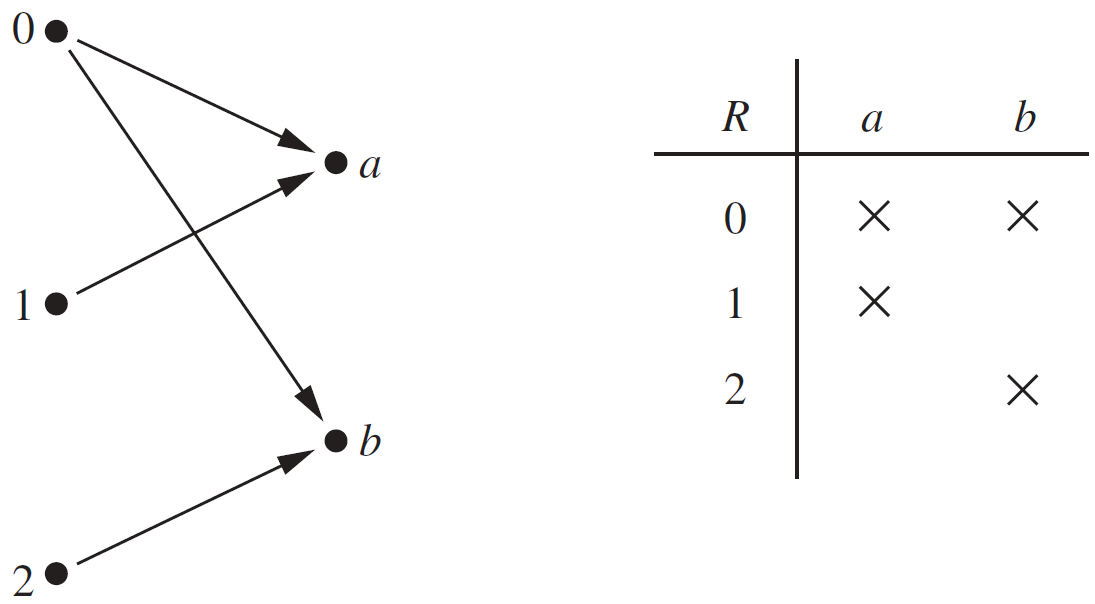
\includegraphics[width=0.5\textwidth]{./img/Displaying-ordered-pairs-Fig1.png}
    \caption{Displaying the ordered pairs in the relation R from Example above.}
    \label{fig:my_label}
\end{figure}

\subsection{Functions as Relations}
Recall that a function $f$ from a set $A$ to a set $B$ assigns exactly one element of $B$ to each element of $A$. The graph of $f$ is the set of ordered pairs $(a, b)$ such that $b = f(a)$. Because the graph of $f$ is a subset of $A \times B$, it is a relation from $A$ to $B$. Moreover, the graph of a function has the property that every element of $A$ is the first element of exactly one ordered pair of the graph.

\subsection{Relations on a Set}
Relations from a set $A$ to itself are of special interest.

\begin{definition}{2}
A \textit{relation on a set $A$} is a relation from $A$ to $A$.
\end{definition}

In other words, a relation on a set $A$ is a subset of $A \times A$.

\begin{example}
Let $A$ be the set $\{1, 2, 3, 4\}$. Which ordered pairs are in the relation $R = \{(a, b) | a \text{ divides } b\}$?

\textbf{Solution}

Because $(a, b)$ is in $R$ if and only if $a$ and $b$ are positive integers not exceeding 4 such that $a$ divides $b$, we see that $R = \{(1, 1), (1, 2), (1, 3), (1, 4), (2, 2), (2, 4), (3, 3), (4, 4)\}$.
\end{example}

\subsection{Properties of Relations}
There are several properties that are used to classify relations on a set. We will introduce the most important of these here.

In some relations an element is always related to itself. For instance, let $R$ be the relation on the set of all people consisting of pairs $(x, y)$ where $x$ and $y$ have the same mother and the same father. Then $x\ R\ x$ for every person $x$.

\begin{definition}{3}
A relation $R$ on a set $A$ is called \textbf{\textit{reflexive}} if $(a, a) \in R$ for every element $a \in A$.
\end{definition}
\textbf{Remark:} Using quantifiers we see that the relation $R$ on the set $A$ is reflexive if $\forall a((a, a) \in R)$, where the universe of discourse is the set of all elements in $A$.

\begin{example}
Consider the following relations on \{1, 2, 3, 4\}:
\begin{align*}
    R_1 &= \{(1, 1), (1, 2), (2, 1), (2, 2), (3, 4), (4, 1), (4, 4)\},\\
    R_2 &= \{(1, 1), (1, 2), (2, 1)\},\\
    R_3 &= \{(1, 1), (1, 2), (1, 4), (2, 1), (2, 2), (3, 3), (4, 1), (4, 4)\},\\
    R_4 &= \{(2, 1), (3, 1), (3, 2), (4, 1), (4, 2), (4, 3)\},\\
    R_5 &= \{(1, 1), (1, 2), (1, 3), (1, 4), (2, 2), (2, 3), (2, 4), (3, 3), (3, 4), (4, 4)\},\\
    R_6 &= \{(3, 4)\}.
\end{align*}
Which of these relations are reflexive?

\textbf{Solution:} The relation $R_3$ and $R_5$ are reflexive because they both contain all pairs of the form $(a,a)$, namely, $(1,1), (2,2), (3, 3)$ and $(4, 4)$.
\end{example}


In some relations an element is related to a second element if and only if the second element is also related to the first element. The relation consisting of pairs $(x, y)$, where $x$ and $y$ are students at your school with at least one common class has this property. Other relations have the property that if an element is related to a second element, then this second element is not related to the first. The relation consisting of the pairs $(x, y)$, where $x$ and $y$ are students at your school, where $x$ has a higher grade point average than $y$ has this property.

\begin{definition}{4}
A relation $R$ on a set $A$ is called \textbf{\textit{symmetric}} if $(b,a) \in R$ whenever $(a,b) \in R$ for all $a, b \in A$. A relation $R$ on a set $A$ such that for all $a, b \in A$, if $(a, b) \in R$ and $(b, a) \in R$, then $a = b$ is called \textbf{\textit{anti-symmetric}}.
\end{definition}
\textbf{Remark:} Using quantifiers, we see that the relation $R$ on the set $A$ is
\begin{itemize}
    \item \textbf{symmetric:} $\forall a \forall b ((a, b) \in R \rightarrow (b, a) \in R)$
    \item \textbf{anti-symmetric:} $\forall a \forall b (((a, b) \in R \land (b, a) \in R) \rightarrow (a = b))$.
\end{itemize}

The terms \textit{symmetric} and \textit{anti-symmetric} are \textbf{not opposites}, because a relation can have both of these properties or may lack both of them. A relation cannot be both symmetric and anti-symmetric if it contains some pair of the form $(a, b)$ in which $a \neq b$.

\textbf{Remark:} Although relatively few of the $2^{n^2}$ relations on a set with $n$ elements are symmetric or anti-symmetric, as counting arguments can show, many important relations have one of these properties.

\begin{example}
Consider the following relations on \{1, 2, 3, 4\}:
\begin{align*}
    R_1 &= \{(1, 1), (1, 2), (2, 1), (2, 2), (3, 4), (4, 1), (4, 4)\},\\
    R_2 &= \{(1, 1), (1, 2), (2, 1)\},\\
    R_3 &= \{(1, 1), (1, 2), (1, 4), (2, 1), (2, 2), (3, 3), (4, 1), (4, 4)\},\\
    R_4 &= \{(2, 1), (3, 1), (3, 2), (4, 1), (4, 2), (4, 3)\},\\
    R_5 &= \{(1, 1), (1, 2), (1, 3), (1, 4), (2, 2), (2, 3), (2, 4), (3, 3), (3, 4), (4, 4)\},\\
    R_6 &= \{(3, 4)\}.
\end{align*}
Which of these relations are symmetric and which are anti-symmetric?

\textbf{Solution:}\\
The relation $R_2$ and $R_3$ are symmetric, because in each case $(b, a)$ belongs to the relation whenever $(a, b)$ does.\\
$R_4, R_5$ and $R_6$ are all anti-symmetric. For each of these relations there is no pair of elements $a$ and $b$ with $a \neq b$ such that both $(a, b)$ and $(b, a)$ belong to the relation.
\end{example}


Let $R$ be the relation consisting of all pairs $(x, y)$ of students at your school, where $x$ has taken more credits than $y$. Suppose that $x$ is related to $y$ and $y$ is related to $z$. This means that $x$ has taken more credits than $y$ and $y$ has taken more credits than $z$. We can conclude that $x$ has taken more credits than $z$, so that $x$ is related to $z$. What we have shown is that $R$ has the \textit{transitive} property, which is defined as follows.

\begin{definition}{5}
A relation $R$ on a set $A$ is called \textbf{\textit{transitive}} if whenever $(a, b) \in R$ and $(b, c) \in R$, then $(a, c) \in R$, for all $a, b, c \in A$.
\end{definition}
\textbf{Remark:} Using quantifiers we see that the relation $R$ on a set $A$ is \textit{transitive} if we have $\forall a \forall b \forall c (((a, b) \in R \land (b, c) \in R) \rightarrow (a, c) \in R)$.

\begin{example}
Consider the following relations on \{1, 2, 3, 4\}:
\begin{align*}
    R_1 &= \{(1, 1), (1, 2), (2, 1), (2, 2), (3, 4), (4, 1), (4, 4)\},\\
    R_2 &= \{(1, 1), (1, 2), (2, 1)\},\\
    R_3 &= \{(1, 1), (1, 2), (1, 4), (2, 1), (2, 2), (3, 3), (4, 1), (4, 4)\},\\
    R_4 &= \{(2, 1), (3, 1), (3, 2), (4, 1), (4, 2), (4, 3)\},\\
    R_5 &= \{(1, 1), (1, 2), (1, 3), (1, 4), (2, 2), (2, 3), (2, 4), (3, 3), (3, 4), (4, 4)\},\\
    R_6 &= \{(3, 4)\}.
\end{align*}
Which of these relations are transitive?

\textbf{Solution:}\\
The relation $R_4, R_5$ and $R_6$ are transitive. For each of these relations,we can show that it is transitive by verifying that if $(a, b)$ and $(b, c)$ belong to this relation, then $(a, c)$ also does.
\end{example}

\subsection{Combining Relations}
Because relations from $A$ to $B$ are subsets of $A \times B$, two relations from $A$ to $B$ can be combined in any way two sets can be combined.

\begin{example}
Let $A = \{1, 2, 3\}$ and $B = \{1, 2, 3, 4\}$. The relations $R_1 = \{(1, 1), (2, 2), (3, 3)\}$ and $R_2 = \{(1, 1), (1, 2), (1, 3), (1, 4)\}$ can be combined to obtain
\begin{align*}
    R_1 \cup R_2 &= \{(1, 1), (1, 2), (1, 3), (1, 4), (2, 2), (3, 3)\},\\
    R_1 \cap R_2 &= \{(1, 1)\},\\
    R_1 \setminus R_2 &= \{(2, 2), (3, 3)\},\\
    R_2 \setminus R_1 &= \{(1, 2), (1, 3), (1, 4)\}.
\end{align*}
\end{example}


There is another way that relations are combined that is analogous to the composition of functions.

\begin{definition}{6}
Let $R$ be a relation from a set $A$ to a set $B$ and $S$ a relation from $B$ to a set $C$. The \textbf{\textit{composite}} of $R$ and $S$ is the relation consisting of ordered pairs $(a, c)$, where $a \in A$, $c \in C$, and for which there exists an element $b \in B$ such that $(a, b) \in R$ and $(b, c) \in S$. We denote the composite of $R$ and $S$ by $S \circ R$.
\end{definition}

Computing the composite of two relations requires that we find elements that are the second element of ordered pairs in the first relation and the first element of ordered pairs in the second relation.

\begin{example}
What is the composite of the relations $R$ and $S$, where $R$ is the relation from $\{1, 2, 3\}$ to $\{1, 2, 3, 4\}$ with $R = \{(1, 1), (1, 4), (2, 3), (3, 1), (3, 4)\}$ and $S$ is the relation from $\{1, 2, 3, 4\}$ to $\{0, 1, 2\}$ with $S = \{(1, 0), (2, 0), (3, 1), (3, 2), (4, 1)\}$?

\textbf{Solution:}

$S \circ R$ is constructed using all ordered pairs in $R$ and ordered pairs in $S$, where the second element of the ordered pair in $R$ agrees with the first element of the ordered pair in $S$. For example, the ordered pairs $(2, 3)$ in $R$ and $(3, 1)$ in $S$ produce the ordered pair $(2, 1)$ in $S \circ R$. Computing all the ordered pairs in the composite, we find
\begin{equation*}
    S \circ R = \{(1, 0), (1, 1), (2, 1), (2, 2), (3, 0), (3, 1)\}.
\end{equation*}
\end{example}

\begin{figure}[h!]
    \centering
    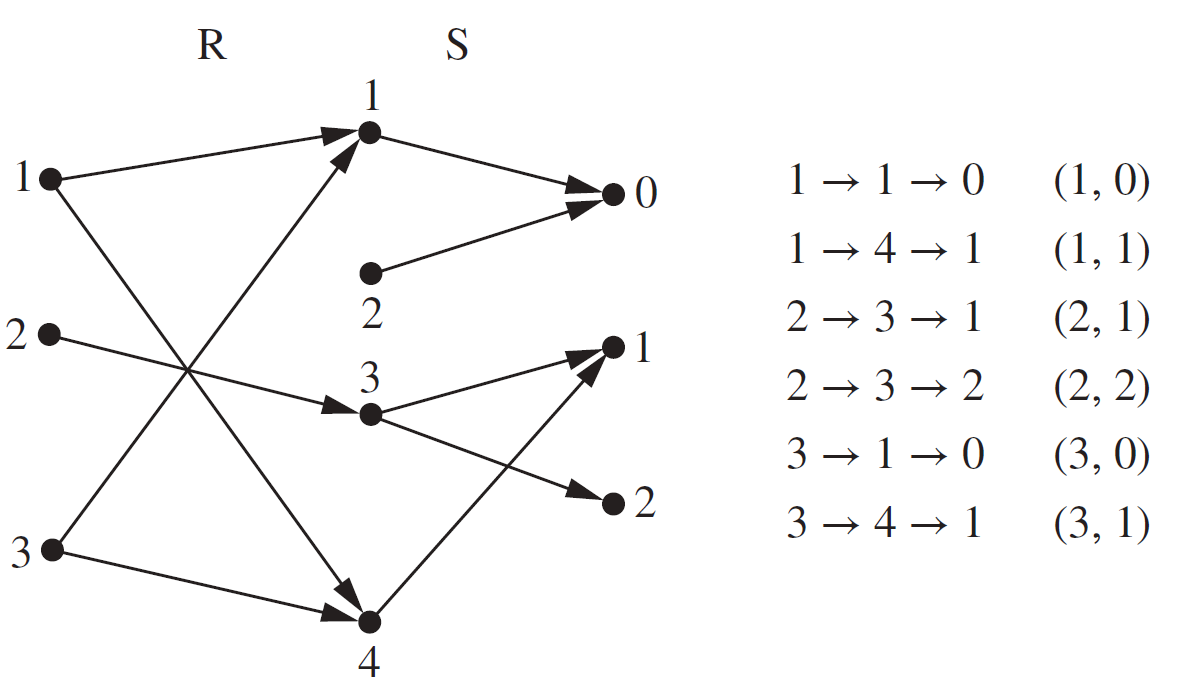
\includegraphics[width=0.5\textwidth]{img/Contructing-S_o_R.png}
    \caption{Constructing $S \circ R$}
    \label{fig:my_label}
\end{figure}


The powers of a relation $R$ can be recursively defined from the definition of a composite of two relations.

\begin{definition}{7}
Let $R$ be a relation on the set $A$. The powers $R^n$, $n = 1, 2, 3, ...$, are defined recursively by
\begin{align*}
    &R^1 = R &\text{and}& &R^{n+1} = R^n \circ R.
\end{align*}
\end{definition}

The definition shows that $R^2 = R \circ R$, $R^3 = R^2 \circ R = (R \circ R) \circ R$, and so on.

\begin{example}
Let $R = \{(1, 1), (2, 1), (3, 2), (4, 3)\}$. Find the powers $R^n$, $n = 2, 3, 4, ...$.

\textbf{Solution:}

Because $R^2 = R \circ R$, we find that $R^2 = \{(1, 1), (2, 1), (3, 1), (4, 2)\}$. Furthermore, because $R^3 = R^2 \circ R$, $R^3 = \{(1, 1), (2, 1), (3, 1), (4, 1)\}$. Additional computation shows that $R^4$ is the same as $R^3$, so $R^4 = \{(1, 1), (2, 1), (3, 1), (4, 1)\}$. It also follows that $R^n = R^3$ for $n =
5, 6, 7, ...$.
\end{example}


The following theorem shows that the powers of a transitive relation are subsets of this relation.
\begin{theorem}{1}
The relation $R$ on a set $A$ is transitive if and only if $R^n \subseteq R$ for $n = 1, 2, 3, ...$.
\end{theorem}

\textbf{Proof:} We first prove the "if" part of the theorem. We supposet that $R^n \subseteq R$ for $n = 1, 2, 3, ...$. In particular, $R^2 \subseteq R$. To see that this implies $R$ is transitive, note that if $(a, b) \in R$ and $(b, c) \in R$, then by the definition of composition, $(a, c) \in R^2$. Because $R^2 \subseteq R$, this means that $(a, c) \in R$. Hence, $R$ is transitive.

We will use mathematical induction to prove the "only if" part of the theorem. Note that this part of the theorem is trivially true for $n = 1$.

Assume that $R^n \subseteq R$, where $n$ is a positive integer. This is the \textit{inductive hypothesis}. To complete the inductive step we must show that this implies that $R^{n+1}$ is also a subset of $R$. To show this, assume that $(a, b) \in R^{n+1}$. Then, because $R^{n+1} = R^n \circ R$, there is an element $x$
with $x \in A$ such that $(a, x) \in R$ and $(x, b) \in R^n$. The inductive hypothesis, namely, that $R^n \subseteq R$, implies that $(x, b) \in R$. Furthermore, because $R$ is transitive, and $(a, x) \in R$ and $(x, b) \in R$, it follows that $(a, b) \in R$. This shows that $R^{n+1} \subseteq R$, completing the proof.


\section{$n$-ary Relations and Their Applications}

\subsection{Introduction}

Relationships among elements of more than two sets often arise. 

For instance, there is a relationship involving the name of a student, the student’s major, and the student’s grade point average. Similarly, there is a relationship involving the airline, flight number, starting point, destination,
departure time, and arrival time of a flight. An example of such a relationship in mathematics involves three integers, where the first integer is larger than the second integer, which is larger than the third. Another example is the betweenness relationship involving points on a line, such that three points are related when the second point is between the first and the third.

We will study relationships among elements from more than two sets in this section. These relationships are called $n$-ary relations. These relations are used to represent computer databases. These representations help us answer queries about the information stored in databases, such as: Which flights land at O’Hare Airport between 3 A.M. and 4 A.M.? Which students at your school are sophomores majoring in mathematics or computer science and have greater than a 3.0 average? 

\subsection{$n$-ary Relations}

We begin with the basic definition on which the theory of relational databases rests.

\begin{definition}{1}
Let $A_1, A_2, ..., A_n$ be sets. An $n$-ary relation on these sets is a subset of $A_1 \times A_2 \times \cdot \cdot \cdot \times A_n$. The sets $A_1, A_2, ..., A_n$ are called the domains of the relation, and $n$ is called its degree.
\end{definition}

\begin{example}
Let $R$ be the relation on $N \times N \times N$ consisting of triples $(a, b, c)$, where $a$, $b$, and $c$ are integers with $a < b < c$. 

Then $(1, 2, 3) \in R$, but $(2, 4, 3) \notin R$. The degree of this relation is $3$. Its domains are all equal to the set of natural numbers.
\end{example}

\begin{example}
Let $R$ be the relation consisting of $5$-tuples $(A, N, S, D, T)$ representing airplane flights, where $A$ is the airline, $N$ is the flight number, $S$ is the starting point, $D$ is the destination, and $T$ is the departure time. 

For instance, if Nadir Express Airlines has flight 963 from Newark to Bangor at 15:00, then (Nadir, 963, Newark, Bangor, 15:00) belongs to $R$. The degree of this relation is 5, and its domains are the set of all airlines, the set of flight numbers, the set of cities, the set of cities (again), and the set of times.
\end{example}

\subsection{Databases and Relations}

The time required to manipulate information in a database \textit{depends on how this information is stored}. The operations of adding and deleting records, updating records, searching for records, and combining records from overlapping databases are performed millions of times each day in a large database. Because of the importance of these operations, various methods for representing databases have been developed. We will discuss one of these methods, called the \textbf{relational data model}, based on the \textit{concept of a relation}.

A database consists of records, which are $n$-tuples, made up of \textbf{fields}. The fields are the entries of the $n$-tuples. 
For instance, a database of student records may be made up of fields containing the name, student number, major, and grade point average of the student. The relational data model represents a database of records as an $n$-ary relation. Thus, student records are represented as 4-tuples of the form (Student name, ID number, Major, GPA).

\textit{Relations used to represent databases are also called \textbf{tables}}, because these relations are often displayed as tables. Each column of the table corresponds to an \textit{attribute} of the database. For instance, a database of students is displayed in Table 1. The attributes of this database
are Student Name, ID Number, Major, and GPA.

\begin{table}[h!]
    \centering
    \caption{Students}
    \begin{tabular}{|l|l|l|l|}
    \hline
        Student\_name    & ID\_number    & Major               & GPA    \\ \hline
        Ackermann        & 231455        & Computer Science    & 3.88   \\ \hline
        Adams            & 888323        & Physics             & 3.45   \\ \hline
        Chou             & 102147        & Computer Science    & 3.49   \\ \hline
        Goodfriend       & 453876        & Mathematics         & 3.45   \\ \hline
        Rao              & 678543        & Mathematics         & 3.90   \\ \hline
        Stevens          & 786576        & Psychology          & 2.99   \\ \hline
    \end{tabular}
    \label{Table 1}
\end{table}

A domain of an $n$-ary relation is called a \textbf{primary key} when the value of the $n$-tuple from this domain determines the $n$-tuple. \textit{That is, a domain is a primary key when no two $n$-tuples in the relation have the same value from this domain}.

\newpage
Records are often added to or deleted from databases. Because of this, the property that a domain is a \textit{primary key is time-dependent}. Consequently, a primary key should be chosen that remains one whenever the database is changed. The current collection of $n$-tuples in a relation is called the \textbf{extension} of the relation. The more permanent part of a database, including the name and attributes of the database, is called its \textbf{intension}. When selecting a primary key, the goal should be to select a key that can serve as a primary key for all possible extensions of the database. To do this, it is necessary to examine the intension of the database to understand the set of possible $n$-tuples that can occur in an extension.

\begin{example}
Which domains are primary keys for the $n$-ary relation displayed in Table 1, assuming that no $n$-tuples will be added in the future?

\textbf{Solution}

Because there is only one 4-tuple in this table for each student name, the domain of student names is a primary key. Similarly, the ID numbers in this table are unique, so the domain of ID numbers is also a primary key. 
However, the domain of major fields of study is \textbf{not} a primary key, because more than one 4-tuple contains the same major field of study. The domain of grade point averages is also not a primary key, because there are two 4-tuples containing the same GPA.
\end{example}

Combinations of domains can also uniquely identify $n$-tuples in an $n$-ary relation. When the values of a set of domains determine an $n$-tuple in a relation, the Cartesian product of these domains is called a \textbf{composite key}.

\begin{example}
Is the Cartesian product of the domain of major fields of study and the domain of GPAs a composite key for the $n$-ary relation from Table 1, assuming that no $n$-tuples are ever added?

\textbf{Solution}

Because no two 4-tuples from this table have both the same major and the same GPA, this Cartesian product is a composite key.
\end{example}

Because primary and composite keys are used to \textit{identify records uniquely in a database}, it is \textit{important that keys remain valid when new records are added to the database}. Hence, checks should be made to ensure that every new record has values that are different in the appropriate field, or fields, from all other records in this table. 
For instance, it makes sense to use the student identification number as a key for student records if no two students ever have the same student identification number. A university should not use the name field as a key, because two students may have the same name.

\subsection{Operations on $n$-ary Relations}

There are a variety of operations on $n$-ary relations that can be used to form new $n$-ary relations. Applied together, these operations can answer queries on databases that ask for all $n$-tuples that satisfy certain conditions.

\subsubsection{Selection}

The most basic operation on an $n$-ary relation is determining all $n$-tuples in the $n$-ary relation that satisfy certain conditions. For example, we may want to find all the records of all computer science majors in a database of student records. We may want to find all students who have a grade point average above 3.5. We may want to find the records of all computer science majors who have a grade point average above 3.5. To perform such tasks we use the \textbf{selection operator}.

\begin{definition}{2}
Let $R$ be an $n$-ary relation and $C$ a condition that elements in $R$ may satisfy. Then the \textit{\textbf{selection operator}} $s_C$ maps the $n$-ary relation $R$ to the $n$-ary relation of all $n$-tuples from $R$ that satisfy the condition $C$.
\end{definition}

\begin{example}
To find the records of computer science majors in the $n$-ary relation R shown in Table 1, we use the operator $s_{C_1}$, where $C_1$ is the condition Major=“Computer Science.” The result is the two 4-tuples (Ackermann, 231455, Computer Science, 3.88) and (Chou, 102147, Computer Science,
3.49). 

Similarly, to find the records of students who have a grade point average above 3.5 in this database, we use the operator $s_{C_2}$, where $C_2$ is the condition GPA $>$ 3.5. The result is the two 4-tuples (Ackermann, 231455, Computer Science, 3.88) and (Rao, 678543, Mathematics, 3.90). 

Finally, to find the records of computer science majors who have a GPA above 3.5, we use the operator $s_{C_3}$, where $C_3$ is the condition (Major = “Computer Science” $\land$ GPA $>$ 3.5). The result consists of the single 4-tuple (Ackermann, 231455, Computer Science, 3.88).
\end{example}

\subsubsection{Projection}

\textbf{Projections} are used to form new $n$-ary relations by deleting the same fields in every record of the relation.

\begin{definition}{3}
The projection $P_{i_1,i_2, ...,i_m}$ where $i_1 < i_2 < \cdot \cdot \cdot < i_m$, maps the $n$-tuple $(a_1, a_2, ..., a_n)$ to the $m$-tuple $(a_{i_1}, a_{i_2}, ..., a_{i_m})$, where $m \leq n$.
\end{definition}

In other words, the projection $P_{i_1,i_2, ...,i_m}$ deletes $n - m$ of the components of an $n$-tuple, leaving the $i_{1}$th, $i_2$th, ..., and $i_m$th components.

\begin{example}
What results when the projection $P_{1,3}$ is applied to the $4$-tuples $(2, 3, 0, 4)$, (Jane Doe, 234111001, Geography, 3.14), and $(a_1, a_2, a_3, a_4)$?

\textbf{Solution}

The projection $P_{1, 3}$ sends these $4$-tuples to $(2, 0)$, (Jane Doe, Geography), and $(a_1, a_3)$, respectively.
\end{example}

Fewer rows may result when a projection is applied to the table for a relation. This happens when some of the $n$-tuples in the relation have identical values in each of the $m$ components of the projection, and only disagree in components deleted by the projection. For instance, consider the following example.

\begin{example}
What is the table obtained when the projection $P_{1, 2}$ is applied to the relation in Table 2?

\textbf{Solution}

Table 3 displays the relation obtained when $P_{1, 2}$ is applied to Table 3. Note that there are fewer rows after this projection is applied.
\end{example}

\begin{table}[!htb]
    %\caption{Global caption}
    \begin{minipage}{.6\linewidth}
    \centering
    \caption{Enrollments}
    \begin{tabular}{|l|l|l|}
    \hline
        Student & Major & Course \\ \hline
        Glauser & Biology & BI 290 \\ \hline
        Glauser & Biology & MS 475 \\ \hline
        Glauser & Biology & PY 410 \\ \hline
        Marcus & Mathematics & MS 511 \\ \hline
        Marcus & Mathematics & MS 603 \\ \hline
        Marcus & Mathematics & CS 322 \\ \hline
        Miller & Computer Science & MS 575 \\ \hline
        Miller & Computer Science & CS 455 \\ \hline
    \end{tabular}
        
    \end{minipage}%
    \begin{minipage}{.4\linewidth}
        \caption{Majors}
        \begin{tabular}{|l|l|}
        \hline
            Student & Major \\ \hline
            Glauser & Biology \\ \hline
            Marcus & Mathematics \\ \hline
            Miller & Computer Science \\ \hline
        \end{tabular}
    \end{minipage} 
\end{table}

\subsubsection{Join}

The \textbf{join} operation is used to combine two tables into one when these tables share some identical fields. For instance, a table containing fields for airline, flight number, and gate, and another table containing fields for flight number, gate, and departure time can be combined into a table containing fields for airline, flight number, gate, and departure time.

\begin{definition}{4}
Let $R$ be a relation of degree $m$ and $S$ a relation of degree $n$. The \textbf{\textit{join}} $J_p(R, S)$, where $p \leq m$ and $p \leq n$, is a relation of degree $m + n - p$ that consists of all $(m + n - p)$-tuples $(a_1, a_2, ..., a_{m-p}, c_1, c_2, ..., c_p, b_1, b_2, ..., b_{n-p})$, where the $m$-tuple $(a_1, a_2, ..., a_{m-p}, c_1, c_2, ..., c_p)$ belongs to $R$ and the $n$-tuple $(c_1, c_2, ..., c_p, b_1, b_2, ..., b_{n-p})$ belongs to $S$.
\end{definition}

In other words, the join operator $J_p$ produces a new relation from two relations by combining all $m$-tuples of the first relation with all $n$-tuples of the second relation, where the last $p$ components of the $m$-tuples agree with the first $p$ components of the $n$-tuples.

\begin{example}
What relation results when the join operator $J_2$ is used to combine the relation displayed in Tables 4 and 5?

\textbf{Solution}

The join $J_2$ produces the relation shown in Table 6.
\end{example}

\begin{table}[!h]
    \begin{minipage}{.45\textwidth}
    \centering
    \caption{Teaching\_assignments}
    \begin{tabular}{|l|l|l|}
    \hline
        Professor & Department & Course\_ \\
        & & number \\ \hline
        Cruz & Zoology & 335 \\ \hline
        Cruz & Zoology & 412 \\ \hline
        Farber & Psychology & 501 \\ \hline
        Farber & Psychology & 617 \\ \hline
        Grammer & Physics & 544 \\ \hline
        Grammer & Physics & 551 \\ \hline
        Rosen & Computer Science & 518 \\ \hline
        Rosen & Mathematics & 575 \\ \hline
    \end{tabular}
        
    \end{minipage}%
    \begin{minipage}{.45\textwidth}
        \caption{Class\_schedule}
        \begin{tabular}{|l|l|l|l|}
        \hline
            Department & Course\_ & Room & Time \\
            & number & & \\ \hline
            Computer Science & 518 & N521 & 2:00 P.M. \\ \hline
            Mathematics & 575 & N502 & 3:00 P.M. \\ \hline
            Mathematics & 611 & N521 & 4:00 P.M. \\ \hline
            Physics & 544 & B505 & 4:00 P.M. \\ \hline
            Psychology & 501 & A100 & 3:00 P.M. \\ \hline
            Psychology & 617 & A110 & 11:00 A.M. \\ \hline
            Zoology & 335 & A100 & 9:00 A.M. \\ \hline
            Zoology & 412 & A100 & 8:00 A.M. \\ \hline
        \end{tabular}
    \end{minipage} 
\end{table}

\begin{table}[!h]
    \centering
    \caption{Teaching\_schedule}
    \begin{tabular}{|l|l|l|l|l|}
        \hline
        Professor & Department & Course\_number & Room & Time \\ \hline
        Cruz & Zoology & 335 & A100 & 9:00 A.M. \\ \hline
        Cruz & Zoology & 412 & A100 & 8:00 A.M. \\ \hline
        Farber & Psychology & 501 & A100 & 3:00 P.M. \\ \hline
        Farber & Psychology & 617 & A110 & 11:00 A.M. \\ \hline
        Grammer & Physics & 544 & B505 & 4:00 P.M. \\ \hline
        Rosen & Computer Science & 518 & N521 & 2:00 P.M. \\ \hline
        Rosen & Mathematics & 575 & N502 & 3:00 P.M. \\ \hline

    \end{tabular}
    \label{tab:my_label}
\end{table}

There are other operators besides projections and joins that produce new relations from existing relations.


\section{Representing Relations}
\setcounter{figure}{0}

\subsection{Introduction}

In this section, and in the remainder of this chapter, all relations we study will be binary relations. Because of this, in this section and in the rest of this chapter, the word "\textit{relation}" will always refer to a binary relation. There are many ways to represent a relation between finite sets. One way is to list its ordered pairs. Another way to represent a relation is to
use a table. 

In this section we will discuss two alternative methods for representing relations. One method uses \textbf{zero–one matrices}. The other method uses
\textit{pictorial representations} called \textbf{directed graphs}.

Generally, matrices are appropriate for the representation of relations in computer programs. On the other hand, people often find the representation of relations using directed graphs useful for understanding the properties of these relations.

\subsection{Representing Relations Using Matrices}

A relation between finite sets can be represented using a \textbf{zero–one matrix}. Suppose that $R$ is a relation from $A = \{a_1, a_2, ..., a_m\}$ to $B = \{b_1, b_2, ..., b_n\}$. (Here the elements of the sets $A$ and $B$ have been listed in a particular, but arbitrary, order. Furthermore, when $A = B$ we use the
same ordering for $A$ and $B$.) The relation $R$ can be represented by the matrix $\textbf{M}_R = [m_{ij}]$, where

$ m_{ij} = 
    \begin{cases}
       1 &\quad\text{if } (a_i, b_j) \in R\\
       0 &\quad\text{if } (a_i, b_j) \notin R\\
    \end{cases}$

\noindent In other words, the zero–one matrix representing $R$ has a 1 as its $(i, j)$ entry when $a_i$ is related to $b_j$, and a 0 in this position if $a_i$ is not related to $b_j$. (Such a representation depends on the orderings used for $A$ and $B$.)

\begin{example}
Suppose that $A = \{1, 2, 3\}$ and $B = \{1, 2\}$. Let $R$ be the relation from $A$ to $B$ containing $(a, b)$ if $a \in A$, $b \in B$, and $a > b$. What is the matrix representing $R$ if $a_1 = 1$, $a_2 = 2$, and $a_3 = 3$, and $b_1 = 1$ and $b_2 = 2$?

\textbf{Solution}

Because $R = \{(2, 1), (3, 1), (3, 2)\}$, the matrix for $R$ is

$\textbf{M}_R =
    \begin{bmatrix}
    0 & 0\\
    1 & 0\\
    1 & 1\\
    \end{bmatrix}$

The $1$s in $\textbf{M}_R$ show that the pairs $(2, 1)$, $(3, 1)$, and $(3, 2)$ belong to $R$. The $0$s show that no other pairs belong to $R$.
\end{example}


The matrix of a relation on a set, which is a square matrix, can be used to determine whether the relation has certain properties. Recall that a relation $R$ on $A$ is \textbf{reflexive} if $(a, a) \in R$ whenever $a \in A$. Thus, $R$ is reflexive if and only if $(a_i, a_i) \in R$ for $i = 1, 2, ..., n$. Hence, $R$ is reflexive if and only if $m_{ii} = 1$, for $i = 1, 2, ..., n$. In other words, $R$ is \textit{reflexive} if all the elements on the main diagonal of $\textbf{M}_R$ are equal to 1, as shown in Figure 1. Note that the elements off the main diagonal can be either 0 or 1.


\begin{figure}[h!]
\begin{minipage}[c]{0.3\textwidth}
    \centering
    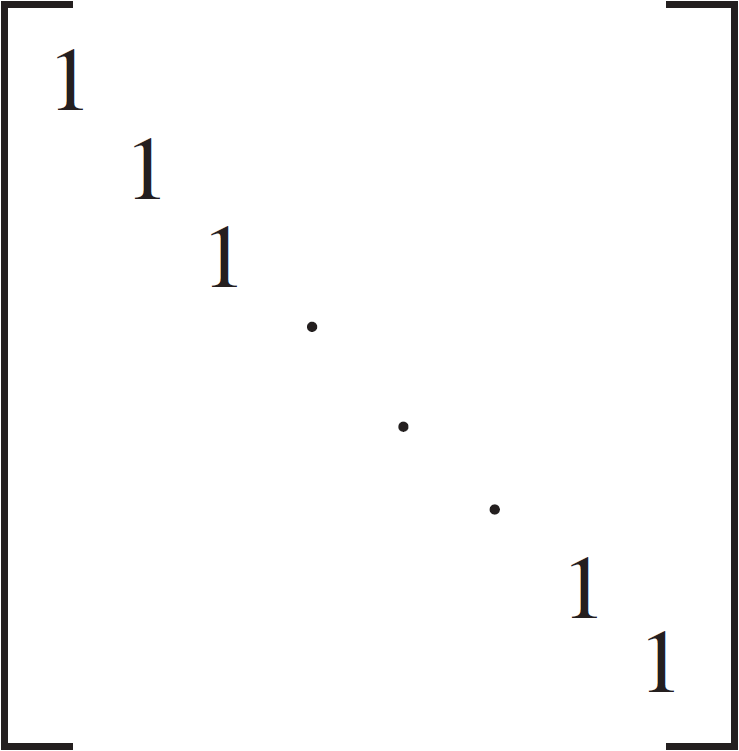
\includegraphics[width=\textwidth]{img/ch9-figure1.png}
    \caption{The zero–one matrix for a reflexive relation.}
\end{minipage}\hfill
\begin{minipage}[c]{0.63\textwidth}
    \centering
    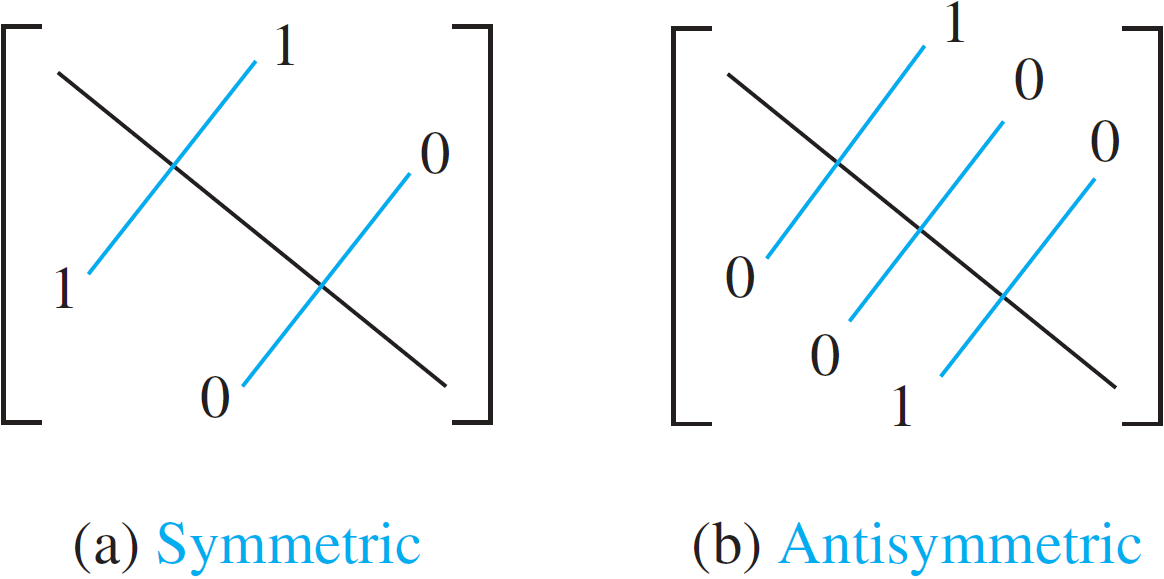
\includegraphics[width=\textwidth]{img/ch9-figure2.png}
    \caption{The zero–one matrices for symmetric and antisymmetric relations}
\end{minipage}\hfill
\end{figure}

\\
The relation $R$ is symmetric if $(a, b) \in R$ implies that $(b, a) \in R$. Consequently, the relation $R$ on the set $A = \{a_1, a_2, ..., a_n\}$ is symmetric if and only if $(a_j, a_i) \in R$ whenever $(a_i, a_j) \in R$. In terms of the entries of $\mathbf{M}_R$, $R$ is symmetric if and only if $m_{ji} = 1$ whenever $m_{ij} = 1$. This also means $m_{ji} = 0$ whenever $m_{ij} = 0$. Consequently, $R$ is symmetric if and only if $m_{ij} = m_{ji}$, for all pairs of integers $i$ and $j$ with $i = 1, 2, ..., n$ and $j = 1, 2, ..., n$.  We see that $R$ is symmetric if and only if
\begin{align*}
    \mathbf{M}_R = (\mathbf{M}_R)^t & & &
\end{align*}

\noindent that is, if $\textbf{M}_R$ is a symmetric matrix. The form of the matrix for a symmetric relation is illustrated in Figure 2(a).\\

The relation $R$ is anti-symmetric if and only if $(a, b) \in R$ and $(b, a) \in R$ imply that $a = b$. Consequently, the matrix of an anti-symmetric relation has the property that if $m_{ij} = 1$ with $i \neq j$, then $m_{ji} = 0$. Or, in other words, either $m_{ij} = 0$ or $m_{ji} = 0$ when $i \neq j$. The form of the matrix for an anti-symmetric relation is illustrated in Figure 2(b).\\

The Boolean operations join and meet can be used to find the matrices
representing the union and the intersection of two relations. Suppose that $R_1$ and $R_2$ are relations on a set $A$ represented by the matrices $\textbf{M}_{R_1}$ and $\textbf{M}_{R_2}$, respectively. The matrix representing
the union of these relations has a 1 in the positions where either $\textbf{M}_{R_1}$ or $\textbf{M}_{R_1}$ has a 1. The matrix representing the intersection of these relations has a 1 in the positions where both $\textbf{M}_{R_1}$ and $\textbf{M}_{R_2}$ have a 1. Thus, the matrices representing the union and intersection of these relations are
\begin{align*}
    &\textbf{M}_{R_1 \cup R_2} = \textbf{M}_{R_1} \lor \textbf{M}_{R_2} &\textbf{M}_{R_1 \cap R_2} = \textbf{M}_{R_1} \land \textbf{M}_{R_2}
\end{align*}

We now turn our attention to determining the matrix for the composite of relations. This matrix can be found using the Boolean product of the matrices for these relations. In particular, suppose that $R$ is a relation from $A$ to $B$ and $S$ is a relation from $B$ to $C$. Suppose that $A$, $B$, and $C$ have $m$, $n$, and $p$ elements, respectively. Let the zero-one matrices for $S \circ R$, $R$, and $S$ be $\textbf{M}_{S \circ R} = [t_{ij}]$, $\textbf{M}_R = [r_{ij}]$, and $\textbf{M}_S = [s_{ij}]$, respectively (these matrices have sizes $m \times p$, $m \times n$, and $n \times p$, respectively). The ordered pair $(a_i, c_j)$ belongs to $S \times R$ if and only if there is an element $b_k$ such that $(a_i, b_k)$ belongs to $R$ and $(b_k, c_j)$ belongs to $S$. It follows that $t_{ij} = 1$ if and only if $r_{ik} = s_{kj} = 1$ for some $k$. 

From the definition of the Boolean product, this means that
\begin{align*}
    \mathbf{M}_{S \circ R} = \mathbf{M}_R \bigodot \mathbf{M}_S & & &
\end{align*}

\noindent The matrix representing the composite of two relations can be used to find the matrix for $\textbf{M}_{R^n}$. In particular,
$\textbf{M}_{R^n} = \textbf{M}_R^{[n]}$,
from the definition of Boolean powers.

\subsection{Representing Relations Using Digraphs}

We have shown that a relation can be represented by listing all of its ordered pairs or by using a zero-one matrix. There is another important way of representing a relation using a pictorial representation. Each element of the set is represented by a point, and each ordered pair is represented using an arc with its direction indicated by an arrow. We use such pictorial representations when we think of relations on a finite set as \textbf{directed graphs}, or \textbf{digraphs}.

\begin{definition}{1}
A \textit{\textbf{directed graph}, or \textbf{digraph}}, consists of a set $V$ of \textit{vertices} (or \textit{nodes}) together with a set $E$ of ordered pairs of elements of $V$ called \textit{edges} (or \textit{arcs}). The vertex a is called the \textit{initial vertex} of the edge $(a, b)$, and the vertex $b$ is called the \textit{terminal vertex} of this edge.
\end{definition}

An edge of the form $(a, a)$ is represented using an arc from the vertex $a$ back to itself. Such an edge is called a \textbf{loop}.

\begin{wrapfigure}{l}{0.25\textwidth}
    \centering
    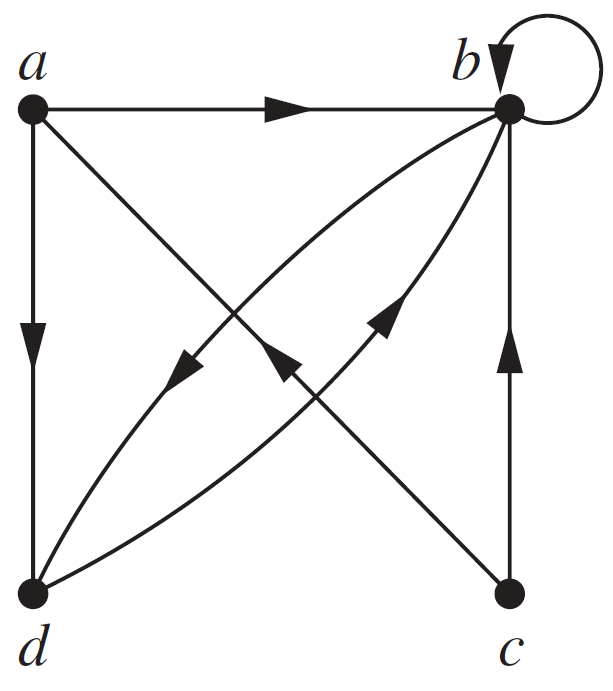
\includegraphics[width=0.25\textwidth]{img/ch9-figure3.png}
    \caption{A directed graph.}
\end{wrapfigure}

The directed graph with vertices $a$, $b$, $c$, and $d$, and edges $(a, b)$, $(a, d)$, $(b, b)$, $(b, d)$, $(c, a)$, $(c, b)$, and $(d, b)$ is displayed in Figure 3.

The relation $R$ on a set $A$ is represented by the directed graph that has the elements of $A$ as its vertices and the ordered pairs $(a, b)$, where $(a, b) \in R$, as edges. This assignment sets up a one-to-one correspondence between the relations on a set $A$ and the directed graphs with $A$ as their set of vertices. Thus, every statement about relations corresponds to a statement about directed graphs, and vice versa. Directed graphs give a visual display of information about relations. As such, they are often used to study relations and their properties. (Note that relations from a set $A$ to a set $B$ can be represented by a directed graph where there is a vertex for each element of $A$ and a vertex for each element of $B$. However, when $A = B$, such representation provides much less insight than the digraph representations described here.)
\\

\begin{example}
The directed graph of the relation $R_1 = \{(1, 1), (1, 3), (2, 1), (2, 3), (2, 4), (3, 1), (3, 2), (4, 1)\}$ on the set $\{1, 2, 3, 4\}$ is shown in Figure 4.
\end{example}

\begin{example}
What are the ordered pairs in the relation $R_2$ represented by the directed graph shown in Figure 5?

\textbf{Solution}
The ordered pairs $(x, y)$ in the relation are $R_2 = \{(1, 3), (1, 4), (2, 1), (2, 2), (2, 3), (3, 1), (3, 3), (4, 1)$, $(4, 3)\}$. Each of these pairs corresponds to an edge of the directed graph, with $(2, 2)$ and $(3, 3)$ corresponding to loops.
\end{example}

\begin{figure*}[h!]
    \centering
    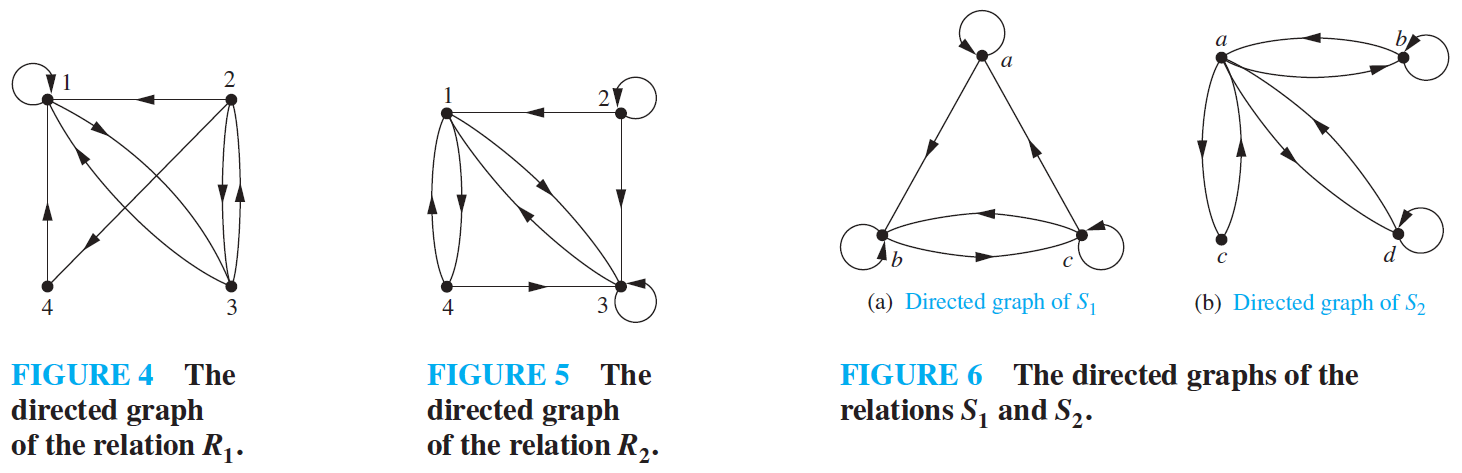
\includegraphics[width=\textwidth]{img/ch9-figure4_5_6.png}
    \label{fig:my_label}
\end{figure*}

\begin{example}
Determine whether the relations for the directed graphs shown in Figure 6 are reflexive, symmetric, anti-symmetric, and/or transitive.

\textbf{Solution}

Because there are loops at every vertex of the directed graph of $S_1$, it is reflexive. The relation $S_1$ is neither symmetric nor anti-symmetric because there is an edge from $a$ to $b$ but not one from $b$ to $a$, but there are edges in both directions connecting $b$ and $c$. Finally, $S_1$ is not transitive because there is an edge from $a$ to $b$ and an edge from $b$ to $c$, but no edge from $a$ to $c$. 

Because loops are not present at all the vertices of the directed graph of $S_2$, this relation is not reflexive. It is symmetric and not anti-symmetric, because every edge between distinct vertices is accompanied by an edge in the opposite direction. It is also not hard to see from the directed graph that $S_2$ is not transitive, because $(c, a)$ and $(a, b)$ belong to $S_2$, but $(c, b)$ does not belong to $S_2$.
\end{example}


\section{Closures of Relations}

\subsection{Introduction}

A computer network has data centers in Boston, Chicago, Denver, Detroit, New York, and San Diego. There are direct, one-way telephone lines from Boston to Chicago, from Boston to Detroit, from Chicago to Detroit, from Detroit to Denver, and from New York to San Diego. Let $R$ be the relation containing $(a, b)$ if there is a telephone line from the data center in $a$ to that in $b$. How can we determine if there is some (possibly indirect) link composed of one or more telephone lines from one center to another? Because not all links are direct, such as the link from Boston to Denver that goes through Detroit, $R$ cannot be used directly to answer this. In the language of relations, $R$ is not transitive, so it does not contain all the pairs that can be linked. As we will show in this section, we can find all pairs of data centers that have a link by constructing a transitive relation $S$ containing $R$ such that $S$ is a subset of every transitive relation containing $R$. Here, $S$ is the smallest transitive relation that contains $R$. This relation is called the \textbf{transitive closure} of $R$.

\subsection{Different Types of Closures}

If $R$ is a relation on a set $A$, it may or may not have some property \textbf{P}, such as \textit{reflexivity, symmetry, \text{or} transitivity}. When $R$ does not enjoy property \textbf{P}, we would like to find the smallest relation $S$ on $A$ with property \textbf{P} that contains $R$.

\begin{definition}{1}
If $R$ is a relation on a set $A$, then the closure of $R$ with respect to \textbf{P}, if it exists, is the relation $S$ on $A$ with property \textbf{P} that contains $R$ and is a subset of every subset of $A \times A$ containing $R$
with property \textbf{P}.
\end{definition}

If there is a relation $S$ that is a subset of every relation containing $R$ with property \textbf{P}, it must be \textit{unique}. To see this, suppose that relations $S$ and $T$ both have property \textbf{P} and are subsets of every relation with property \textbf{P} that contains $R$. Then, $S$ and $T$ are subsets of each other, and so are equal. Such a relation, if it exists, is the smallest relation with property \textbf{P} that contains $R$ because it is a subset of every relation with property \textbf{P} that contains $R$.

We will show how \textit{reflexive, symmetric}, and \textit{transitive} closures of relations can be found.

\subsubsection{Reflexive Closure}

The relation $R = \{(1, 1), (1, 2), (2, 1), (3, 2)\}$ on the set $A = \{1, 2, 3\}$ is not \textit{reflexive}. How can we produce a reflexive relation containing $R$ that is as small as possible? This can be done by adding $(2, 2)$ and $(3, 3)$ to $R$, because these are the only pairs of the form $(a, a)$ that are not in $R$. This new relation contains $R$. Furthermore, any reflexive relation that contains $R$ must also contain $(2, 2)$ and $(3, 3)$. Because this relation contains $R$, is reflexive, and is contained within every reflexive relation that contains $R$, it is called the \textbf{reflexive closure} of $R$.\\


As this example illustrates, given a relation $R$ on a set $A$, the reflexive closure of $R$ can be formed by adding to $R$ all pairs of the form $(a, a)$ with $a \in A$, not already in $R$. The addition of these pairs produces a new relation that is \textit{reflexive}, contains $R$, and is contained within any reflexive relation containing $R$. We see that the reflexive closure of $R$ equals $R \cup \Delta$, where $\Delta = \{(a, a)\ |\ a \in A\}$ is the diagonal relation on $A$.

\begin{example}
What is the reflexive closure of the relation $R = \{(a, b)\ |\ a < b\}$ on the set of integers?

\textbf{Solution:}

The reflexive closure of $R$ is $R \cup \Delta = \{(a, b)\ |\ a < b\} \cup \{(a, a)\ |\ a \in \mathbf{Z}\} = \{(a, b)\ |\ a \leq b\}$.
\end{example}


\subsubsection{Symmetric Closure}

The relation $\{(1, 1), (1, 2), (2, 2), (2, 3), (3, 1), (3, 2)\}$ on $\{1, 2, 3\}$ is not symmetric. How can we produce a symmetric relation that is as small as possible and contains R? To do this, we need only add $(2, 1)$ and $(1, 3)$, because these are the only pairs of the form $(b, a)$ with $(a, b) \in R$ that are not in $R$. This new relation is \textit{symmetric} and contains $R$. Furthermore, \textit{any} symmetric relation that contains $R$ must contain this new relation, because a symmetric relation that contains $R$ must contain $(2, 1)$ and $(1, 3)$. Consequently, this new relation is called the \textbf{symmetric closure} of $R$.\\

As this example illustrates, the symmetric closure of a relation $R$ can be constructed by adding all ordered pairs of the form $(b, a)$, where $(a, b)$ is in the relation, that are not already present in $R$. Adding these pairs produces a relation that is \textit{symmetric}, that contains $R$, and that is contained in any symmetric relation that contains $R$. The \textit{symmetric closure} of a relation can be constructed by \textit{\textbf{taking the union of a relation with its inverse}}; that is, $R \cup R^{-1}$ is the symmetric closure of R, where $R^{-1} = \{(b, a)\ |\ (a, b) \in R\}$.

\begin{example}
What is the symmetric closure of the relation $R = \{(a, b)\ |\ a > b\}$ on the set of positive integers?

\textbf{Solution:}

The symmetric closure of $R$ is the relation

$R \cup R^{-1} = \{(a, b)\ |\ a > b\} \cup \{(b, a)\ |\ a > b\} = \{(a, b)\ |\ a \neq b\}$.
\end{example}

\subsection{Paths in Directed Graph}

We will see that representing relations by directed graphs helps in the construction of \textit{transitive closures}. We now introduce some terminology that we will use for this purpose. A path in a directed graph is obtained by traversing along edges (in the same direction as indicated by the arrow on the edge).

\begin{definition}{2}
A path from $a$ to $b$ in the directed graph $G$ is a sequence of edges $(x_0, x_1)$, $(x_1, x_2)$, $(x_2, x_3)$, ..., $(x_{n-1}, x_n)$ in $G$, where $n$ is a non-negative integer, and $x_0 = a$ and $x_n = b$, that is, a sequence of edges where the terminal vertex of an edge is the same as the initial vertex in the next edge in the path. This path is denoted by $x_0, x_1, x_2, ..., x_{n-1}, x_n$ and has length $n$. We view the empty set of edges as a path of length zero from $a$ to $a$. A path of length $n \geq 1$ that begins and ends at the same vertex is called a \textit{\textbf{circuit}} or \textit{\textbf{cycle}}.
\end{definition}

A path in a directed graph can pass through a vertex more than once. Moreover, an edge in a directed graph can occur more than once in a path.


The term \textit{path} also applies to relations. Carrying over the definition from directed graphs to relations, there is a \textbf{path} from $a$ to $b$ in $R$ if there is a sequence of elements $a, x_1, x_2, ..., x_{n-1}, b$ with $(a, x_1) \in R$, $(x_1, x_2) \in R$, ..., and $(x_{n-1}, b) \in R$. Theorem 1 can be obtained from the definition of a path in a relation.

\begin{theorem}{1}
Let $R$ be a relation on a set $A$. There is a path of length $n$, where $n$ is a positive integer, from $a$ to $b$ if and only if $(a, b) \in R^n$.
\end{theorem}

\textbf{Proof:} We will use mathematical induction. By definition, there is a path from $a$ to $b$ of length one if and only if $(a, b) \in R$, so the theorem is true when $n = 1$.

Assume that the theorem is true for the positive integer $n$. This is the inductive hypothesis. There is a path of length $n + 1$ from $a$ to $b$ if and only if there is an element $c \in A$ such that there is a path of length one from $a$ to $c$, so $(a, c) \in R$, and a path of length $n$ from $c$ to $b$, that is, $(c, b) \in R^n$. Consequently, by the inductive hypothesis, there is a path of length $n + 1$ from $a$ to $b$ if and only if there is an element $c$ with $(a, c) \in R$ and $(c, b) \in R^n$. But there is such an element if and only if $(a, b) \in R^{n+1}$. Therefore, there is a path of length $n + 1$ from $a$ to $b$ if and only if $(a, b) \in R^{n+1}$. This completes the proof.


\subsection{Transitive Closures}

We now show that finding the \textit{transitive closure} of a relation is equivalent to determining which pairs of vertices in the associated directed graph are connected by a path. With this in mind, we define a new relation.

\begin{definition}{3}
Let $R$ be a relation on a set $A$. The connectivity relation $R^*$ consists of the pairs $(a, b)$ such that there is a path of length at least one from $a$ to $b$ in $R$.
\end{definition}

Because $R^n$ consists of the pairs $(a, b)$ such that there is a path of length $n$ from $a$ to $b$, it follows that $R^*$ is the union of all the sets $R^n$. In other words,

\begin{equation*}
    R^* = \bigcup^{\infty}_{n=1} R^n
\end{equation*}

The connectivity relation is useful in many models.

\begin{example}
Let $R$ be the relation on the set of all people in the world that contains $(a, b)$ if $a$ has met $b$. What is $R^n$, where $n$ is a positive integer greater than one? What is $R^*$?

\textbf{Solution:}

The relation $R^2$ contains $(a, b)$ if there is a person $c$ such that $(a, c) \in R$ and $(c, b) \in R$, that is, if there is a person $c$ such that $a$ has met $c$ and $c$ has met $b$. Similarly, $R^n$ consists of those pairs $(a, b)$ such that there are people $x_1, x_2, ..., x_{n-1}$ such that $a$ has met $x_1$, $x_1$ has met $x_2$ , ..., and $x_{n-1}$ has met $b$. 

The relation $R^*$ contains $(a, b)$ if there is a sequence of people, starting with $a$ and ending with $b$, such that each person in the sequence has met the next person in the sequence. (There are many interesting conjectures about $R^*$.
\end{example}

Theorem 2 shows that the \textit{transitive closure} of a relation and the \textit{associated connectivity} relation are the same.

\begin{theorem}{2}
The transitive closure of a relation $R$ equals the connectivity relation $R^*$.
\end{theorem}

\textbf{Proof:} Note that $R^*$ contains $R$ by definition. To show that $R^*$ is the transitive closure of $R$ we must also show that $R^*$ is transitive and that $R^* \subseteq S$ whenever $S$ is a transitive relation that contains $R$.

First, we show that $R^*$ is transitive. If $(a, b) \in R^*$ and $(b, c) \in R^*$, then there are paths from $a$ to $b$ and from $b$ to $c$ in $R$. We obtain a path from $a$ to $c$ by starting with the path from $a$ to $b$ and following it with the path from $b$ to $c$. Hence, $(a, c) \in R^*$. It follows that $R^*$ is transitive.\\

Now suppose that $S$ is a transitive relation containing $R$. Because $S$ is transitive, $S^n$ also is transitive and $S^n \subseteq S$. Furthermore, because

\begin{equation*}
    S^* = \bigcup^{\infty}_{k=1} S^k
\end{equation*}

\noindent and $S^k \subseteq S$, it follows that $S^* \subseteq S$. Now note that if $R \subseteq S$, then $R^* \subseteq S^*$, because any path in $R$ is also a path in $S$. Consequently, $R^* \subseteq S^* \subseteq S$. Thus, any transitive relation that contains $R$ must also contain $R^*$. Therefore, $R^*$ is the transitive closure of $R$.

Now that we know that the transitive closure equals the connectivity relation, we turn our attention to the problem of computing this relation. We do not need to examine arbitrarily long paths to determine whether there is a path between two vertices in a finite directed graph. As Lemma 1 shows, it is sufficient to examine paths containing no more than $n$ edges, where $n$ is the number of elements in the set.

\newpage
\begin{mybox}{violet}{\textbf{Lemma 1}}
Let $A$ be a set with $n$ elements, and let $R$ be a relation on $A$. If there is a path of length at least one in $R$ from $a$ to $b$, then there is such a path with length not exceeding $n$. Moreover, when $a \neq b$, if there is a path of length at least one in $R$ from $a$ to $b$, then there is such a path with length not exceeding $n - 1$.
\end{mybox}

\textbf{Proof:} Suppose there is a path from $a$ to $b$ in $R$. Let $m$ be the length of the shortest such path. Suppose that $x_0, x_1, x_2, ..., x_{m-1}, x_m$, where $x_0 = a$ and $x_m = b$, is such a path. 

Suppose that $a = b$ and that $m > n$, so that $m \geq n + 1$. By the pigeonhole principle, because there are $n$ vertices in $A$, among the $m$ vertices $x_0, x_1, ..., x_{m-1}$, at least two are equal (see
Figure 2).

\begin{figure}[!h]
    \centering
    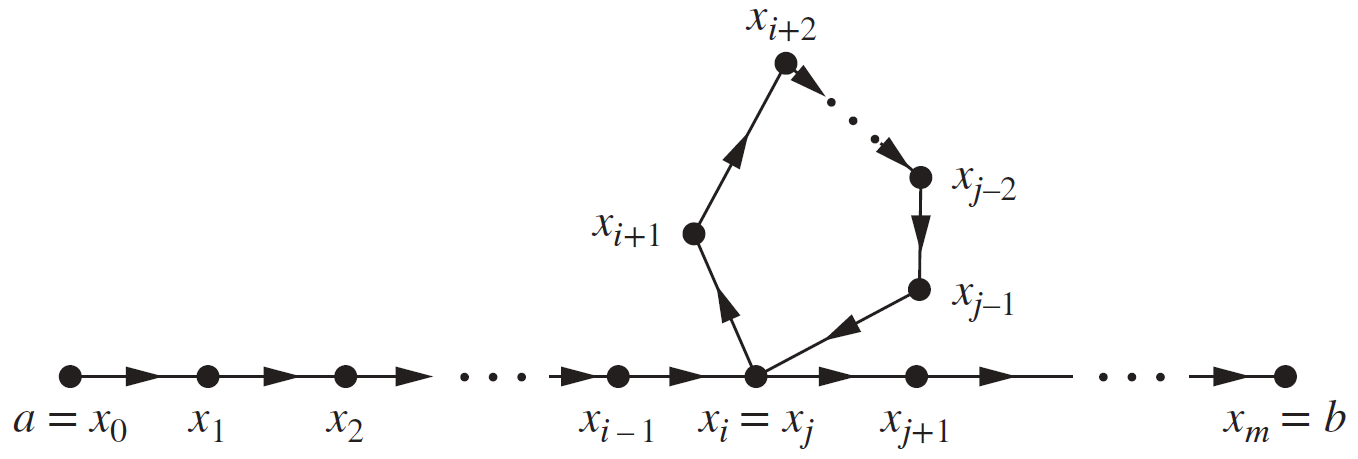
\includegraphics[width=.8\textwidth]{img/ch9.4-figure2.png}
    \label{fig:my_label}
\end{figure}

Suppose that $x_i = x_j$ with $0 \leq i < j \leq m - 1$. Then the path contains a circuit from $x_i$ to itself. This circuit can be deleted from the path from $a$ to $b$, leaving a path, namely, $x_0, x_1, ..., x_i, x_{j+1}, ..., x_{m-1}, x_m$, from $a$ to $b$ of shorter length. Hence, the path of shortest length must have length less than or equal to $n$.\\

From Lemma 1, we see that the transitive closure of $R$ is the union of $R$, $R^2$, $R^3$, ..., and $R^n$. This follows because there is a path in $R^*$ between two vertices if and only if there is a path between these vertices in $R^i$, for some positive integer $i$ with $i \leq n$. Because
\begin{align*}
    R^* = R \cup R^2 \cup R^3 \cup \cdot \cdot \cdot \cup R^n & & &
\end{align*}

\noindent and the zero-one matrix representing a union of relations is the join of the zero-one matrices of these relations, \textit{the zero-one matrix for the transitive closure} is \textit{the join of the zero-one matrices
of the first $n$ powers of the zero-one matrix of $R$}.

\begin{theorem}{3}
Let $\mathbf{M}_R$ be the zero-one matrix of the relation $R$ on a set with $n$ elements. Then the zero-one matrix of the transitive closure $R^*$ is
\begin{align*}
    \mathbf{M}_{R^*} = \mathbf{M}_R \lor \mathbf{M}_R^{[2]} \lor \mathbf{M}_R^{[3]} \lor \cdot \cdot \cdot \lor \mathbf{M}_R^{[n]}    
\end{align*}
\end{theorem}

\newpage
\begin{example}
Find the zero-one matrix of the transitive closure of the relation $R$ where

\begin{equation*}
\textbf{M}_R = 
    \begin{bmatrix}
    1 & 0 & 1\\
    0 & 1 & 0\\
    1 & 1 & 0
    \end{bmatrix}
\end{equation*}

By Theorem 3, it follows that the zero-one matrix of $R^*$ is

\begin{equation*}
    \textbf{M}_{R^*} = \textbf{M}_{R} \lor \textbf{M}_{R}^{[2]} \lor \textbf{M}_{R}^{[3]}.
\end{equation*}

Because

\begin{align*}
    &\textbf{M}_R^{[2]} = 
    \begin{bmatrix}
    1 & 1 & 1\\
    0 & 1 & 0\\
    1 & 1 & 1
    \end{bmatrix}
    & \text{ and } &
    & \textbf{M}_R^{[3]} = 
    \begin{bmatrix}
    1 & 1 & 1\\
    0 & 1 & 0\\
    1 & 1 & 1
    \end{bmatrix}
\end{align*}

it follows that

\begin{equation*}
    \textbf{M}_{R^*} = 
    \begin{bmatrix}
    1 & 0 & 1\\
    0 & 1 & 0\\
    1 & 1 & 0
    \end{bmatrix} \lor
    \begin{bmatrix}
    1 & 1 & 1\\
    0 & 1 & 0\\
    1 & 1 & 1
    \end{bmatrix} \lor
    \begin{bmatrix}
    1 & 1 & 1\\
    0 & 1 & 0\\
    1 & 1 & 1
    \end{bmatrix} =
    \begin{bmatrix}
    1 & 1 & 1\\
    0 & 1 & 0\\
    1 & 1 & 1
    \end{bmatrix}
\end{equation*}
\end{example}

Theorem 3 can be used as a basis for an algorithm for computing the matrix of the relation $R^*$. To find this matrix, the successive Boolean powers of $\mathbf{M}_R$, up to the $n^{th}$ power, are computed. As each power is calculated, its join with the join of all smaller powers is formed. When this is done with the $n^{th}$ power, the matrix for $R^*$ has been found. This procedure is displayed as Algorithm 1

\begin{algorithm}
\caption{A Procedure for Computing the Transitive Closure}
\begin{algorithmic}[1]
\Procedure{transitive closure}{$M_R$ : zero-one $n \times n$ matrix}
\State A := $M_R$
\State B := A
\For {i := 2 to $n$}
    \State A := A $\bigodot$ $M_R$
    \State B:= B $\lor$ A
\EndFor
\State \textbf{return B} \{\textbf{B} is the zero-one matrix for $R^*$\}
\EndProcedure
\end{algorithmic}
\end{algorithm}

We can easily find the number of bit operations used by Algorithm 1 to determine the transitive closure of a relation. Computing the Boolean powers $\textbf{M}_R, \textbf{M}_R^{[2]}, \cdot \cdot \cdot, \textbf{M}_R^{[n]}$ requires that $n-1$ Boolean products of $n \times n$ zero-one matrices be found. Each of these Boolean products can be found using $n^2(2n-1)$ bit operations. Hence, these products can be computed using $n^2(2n-1)(n-1)$ bit operations.

To find $\textbf{M}_{R^*}$ from the $n$ Boolean powers of $\textbf{M}_R$, $n-1$ joins of zero–one matrices need to be found. Computing each of these joins uses $n^2$ bit operations. Hence, $(n-1)n^2$ bit operations are used in this part of the computation. Therefore, when Algorithm 1 is used, the matrix of the transitive closure of a relation on a set with $n$ elements can be found using $n^2(2n-1)(n-1) + (n-1)n^2 = 2n^3(n-1)$, which is $O(n^4)$ bit operations.

\newpage
\subsection{Warshall’s Algorithm}

\textit{(This part may be read from text book. Some part of the this subsection can be read below)}.

\noindent Warshall’s algorithm is an efficient method for computing the transitive closure of a relation. Algorithm 1 can find the transitive closure of a relation on a set with $n$ elements using $2n^3(n−1)$ bit operations. However, the transitive closure can be found by Warshall’s algorithm using only $2n^3$ bit operations.

\begin{algorithm}
\caption{Warshall Algorithm}
\begin{algorithmic}
\Procedure{$Warshall$}{$\mathbf{M}_R$: $n \times n$ zero-one matrix}
\State $\mathbf{W}$ := $\mathbf{M}_R$
\For{$k$ := 1 \textbf{to} $n$}
\For{$i$ := 1 \textbf{to} $n$}
\For{$j$ := 1 \textbf{to} $n$}
\State $w_{ij}$ := $w_{ij} \lor (w_{ik} \land w_{kj})$
\EndFor
\EndFor
\EndFor
\State \Return{$\mathbf{W}$}\ \{$\mathbf{W} = [w_{ij}]$ is $\mathbf{M}_{R^*}$\}
\EndProcedure
\end{algorithmic}
\end{algorithm}

The computational complexity ofWarshall’s algorithm can easily be computed in terms of bit operations. The total number of bit operations used is $n \cdot 2n^2 = 2n^3$

\section{Equivalence Relations}

\subsection{Introduction}

In some programming languages the names of variables can contain an unlimited number of characters. However, there is a limit on the number of characters that are checked when a compiler determines whether two variables are equal. For instance, in traditional C, only the first eight characters of a variable name are checked by the compiler. (These characters are uppercase or lowercase letters, digits, or underscores.) Consequently, the compiler considers strings longer than eight characters that agree in their first eight characters the same. Let $R$ be the relation on the set of strings of characters such that $s R t$, where $s$ and $t$ are two strings, if $s$ and $t$ are at least eight characters long and the first eight characters of $s$ and $t$ agree, or $s = t$. It is easy to see that $R$ is reflexive, symmetric, and transitive. Moreover, $R$ divides the set of all strings into classes, where all strings in a particular class are considered the same by a compiler for traditional C.

The integers $a$ and $b$ are related by the “congruence modulo 4” relation when 4 divides $a-b$. We will show later that this relation is reflexive, symmetric, and transitive. It is not hard to see that $a$ is related to $b$ if and only if $a$ and $b$ have the same remainder when divided by 4. It follows that this relation splits the set of integers into four different classes. When we care only what remainder an integer leaves when it is divided by 4, we need only know which class it is in, not its particular value.

These two relations, $R$ and congruence modulo 4, are examples of equivalence relations, namely, relations that are reflexive, symmetric, and transitive. In this section we will show that such relations split sets into disjoint classes of equivalent elements. Equivalence relations arise whenever we care only whether an element of a set is in a certain class of elements, instead of caring about its particular identity.

\subsection{Equivalence Relations}

In this section we will study relations with a particular combination of properties that allows them to be used to relate objects that are similar in some way.

\begin{definition}{1}
A relation on a set $A$ is called an \textit{\textbf{equivalence relation}} if it is \textit{reflexive}, \textit{symmetric}, and \textit{transitive}.
\end{definition}

Equivalence relations are important throughout mathematics and computer science. One reason for this is that in an equivalence relation, when two elements are related it makes sense to say they are equivalent.

\begin{definition}{2}
Two elements $a$ and $b$ that are related by an equivalence relation are called \textit{\textbf{equivalent}}. The notation $a \sim b$ is often used to denote that $a$ and $b$ are equivalent elements with respect to a particular equivalence relation.
\end{definition}

For the notion of equivalent elements to make sense, every element should be equivalent to itself, as the reflexive property guarantees for an equivalence relation. It makes sense to say that $a$ and $b$ are related (not just that $a$ is related to $b$) by an equivalence relation, because when $a$ is related to $b$, by the symmetric property, $b$ is related to $a$. Furthermore, because an equivalence relation is transitive, if $a$ and $b$ are equivalent and $b$ and $c$ are equivalent, it follows that $a$ and $c$ are equivalent.

\begin{example}
Let $R$ be the relation on the set of integers such that $a R b$ if and only if $a = b$ or $a = -b$.

$R$ is reflexive, symmetric, and transitive. It follows that $R$ is an equivalence relation.
\end{example}

One of the most widely used equivalence relations is congruence modulo $m$, where $m$ is an integer greater than 1.

\begin{example}[Congruence Modulo $m$]
Let $m$ be an integer with $m > 1$. Show that the relation $R = \{(a, b)\ |\ a \equiv b\ (\bmod{\ m})\}$ is an equivalence relation on the set of integers.

\textbf{Solution:}

Because $a-a = 0$ is an integer for all real numbers $a$, $a R a$ for all real numbers $a$. Hence, $R$ is reflexive.\\
Now suppose that $a R b$. Then $a-b$ is an integer, so $b-a$ is also an integer. Hence, $b R a$. It follows that $R$ is symmetric.\\
If $a R b$ and $b R c$, then $a-b$ and $b-c$ are integers. Therefore, $a-c = (a-b) + (b-c)$ is also an integer. Hence, $a R c$. Thus, $R$ is transitive.\\
Consequently, $R$ is an equivalence relation.
\end{example}

\begin{example}
Show that the "divides" relation on the set of positive integers in not an equivalence relation.

\textbf{Solution:}

We know that the "divides" relation is reflexive and transitive. However, we also know that this relation is not symmetric (for instance, $2 \mid 4$ but $4 \centernot{|} 2$). We conclude that the "divides" relation on the set of positive integers is not an equivalence relation.
\end{example}

\subsection{Equivalence Classes}

Let $A$ be the set of all students in your school who graduated from high school. Consider the relation $R$ on $A$ that consists of all pairs $(x, y)$, where $x$ and $y$ graduated from the same high school. Given a student $x$, we can form the set of all students equivalent to $x$ with respect to $R$. This set consists of all students who graduated from the same high school as $x$ did. This subset of $A$ is called an equivalence class of the relation.

\begin{definition}{3}
Let $R$ be an equivalence relation on a set $A$. The set of all elements that are related to an element $a$ of $A$ is called the equivalence class of $a$. The equivalence class of $a$ with respect to $R$ is denoted by $[a]_R$. When only one relation is under consideration, we can delete the subscript $R$ and write $[a]$ for this equivalence class.
\end{definition}

\noindent In other words, if $R$ is an equivalence relation on a set $A$, the equivalence class of the element $a$ is
\begin{align*}
    [a]_R = \{s\ |\ (a, s) \in R\} & & &    
\end{align*}

\noindent If $b \in [a]_R$, then $b$ is called a \textbf{representative} of this equivalence class. Any element of a class can be used as a representative of this class. That is, there is nothing special about the particular
element chosen as the representative of the class.

\begin{example}
What is the equivalence class of an integer for the equivalence relation of the relation $R$ on the set of integers such that $a R b$ if and only if $a = b$ or $a = -b$?

\textbf{Solution:}

Because an integer is equivalent to itself and its negative in this equivalence relation, it follows that $[a] = \{-a, a\}$. This set contains two distinct integers unless $a = 0$. For instance, $[7] = \{-7, 7\},\ [-5] = \{-5, 5\}$, and $[0] = \{0\}$.
\end{example}

\noindent \textbf{Example}: What are the equivalence classes of 0, 1, 2, and 3 for congruence modulo 4?

\noindent \textbf{Solution:}

The equivalence class of 0 contains all integers a such that $a \equiv 0 (\bmod{\ 4})$. The integers in this class are those divisible by 4. Hence, the equivalence class of 0 for this relation is
\begin{align*}
    [0] = \{..., -8, -4, 0, 4, 8, ...\} & & & & & & & & & &
\end{align*}

The equivalence class of 1 contains all the integers a such that $a \equiv 1 (\bmod{ 4})$. The integers in this class are those that have a remainder of 1 when divided by 4. Hence, the equivalence class of 1 for this relation is
\begin{align*}
    [1] = \{..., -7, -3, 1, 5, 9, ...\} & & & & & & & & & &
\end{align*}

The equivalence class of 2 contains all the integers a such that $a \equiv 2 (\bmod{ 4})$. The integers in this class are those that have a remainder of 2 when divided by 4. Hence, the equivalence class of 2 for this relation is
\begin{align*}
    [2] = \{..., -6, -2, 2, 6, 10, ...\} & & & & & & & & & &
\end{align*}

The equivalence class of 3 contains all the integers a such that $a \equiv 3 (\bmod{ 4})$. The integers in this class are those that have a remainder of 3 when divided by 4. Hence, the equivalence class of 3 for this relation is
\begin{align*}
    [3] = \{..., -5, -1, 3, 7, 11, ...\} & & & & & & & & & &.
\end{align*}

Note that every integer is in exactly one of the four equivalence classes and that the integer $n$ is in the class containing $n \bmod 4$

The equivalence classes of 0, 1, 2, and 3 with respect to congruence modulo 4 were found. The above example can easily be generalized, replacing 4 with any positive integer $m$. The equivalence classes of the relation congruence modulo $m$ are called the \textbf{congruence classes modulo $m$}. The congruence class of an integer $a$ modulo $m$ is denoted by $[a]_m$, so $[a]_m = \{..., a - 2m, a - m, a, a + m, a + 2m, ...\}$. For instance, from the above example, we have $[0]_4 = \{..., -8, -4, 0, 4, 8, ...\}$, $[1]_4 = \{..., -7, -3, 1, 5, 9, ...\}$, $[2]_4 = \{..., -6, -2, 2, 6, 10,...\}$, and $[3]_4 = \{..., -5, -1, 3, 7, 11, ...\}$.

\subsection{Equivalence Classes and Partitions}

Let $A$ be the set of students at your school who are majoring in exactly one subject, and let $R$ be the relation on $A$ consisting of pairs $(x, y)$, where $x$ and $y$ are students with the same major. Then $R$ is an equivalence relation. We can see that $R$ splits all students in $A$ into a collection of disjoint subsets, where each subset contains students with a specified major. For instance, one subset contains all students majoring (just) in computer science, and a second subset contains all students majoring in history. Furthermore, these subsets are equivalence classes of $R$. This example illustrates how the equivalence classes of an equivalence relation partition a set into disjoint, nonempty subsets. We will make these notions more
precise in the following discussion.

Let $R$ be a relation on the set $A$. Theorem 1 shows that the equivalence classes of two elements of $A$ are either identical or disjoint.

\begin{theorem}{1}
Let $R$ be an equivalence relation on a set $A$. These statements for elements $a$ and $b$ of $A$ are equivalent:
\begin{align*}
    &(i) aRb& &(ii) [a] = [b]& &(iii) [a] \cap [b] \neq \emptyset    
\end{align*}
\end{theorem}

\textbf{Proof:} We first show that $(i)$ implies $(ii)$. Assume that $a R b$. We will prove that $[a] = [b]$ by showing $[a] \subseteq [b]$ and $[b] \subseteq [a]$. Suppose $c \in [a]$. Then $a R c$. Because $a R b$ and $R$ is symmetric, we know that $b R a$. Furthermore, because $R$ is transitive and $b R a$ and $a R c$, it follows that $b R c$. Hence, $c \in [b]$. This shows that $[a] \subseteq [b]$. The proof that $[b] \subseteq [a]$ is similar.

Second, we will show that $(ii)$ implies $(iii)$. Assume that $[a] = [b]$. It follows that $[a] \cap [b] \neq \emptyset$ because $[a]$ is nonempty (because $a \in [a]$ because $R$ is reflexive).

Next, we will show that $(iii)$ implies $(i)$. Suppose that $[a] \cap [b] \neq \emptyset$. Then there is an element $c$ with $c \in [a]$ and $c \in [b]$. In other words, $a R c$ and $b R c$. By the symmetric property, $c R b$. Then by transitivity, because $a R c$ and $c R b$, we have $a R b$.

Because $(i)$ implies $(ii)$, $(ii)$ implies $(iii)$, and $(iii)$ implies $(i)$, the three statements, $(i)$, $(ii)$, and $(iii)$, are equivalent.\\

We are now in a position to show how an equivalence relation \textit{partitions} a set. Let $R$ be an equivalence relation on a set $A$. The union of the equivalence classes of $R$ is all of $A$, because an element a of $A$ is in its own equivalence class, namely, $[a]_R$. In other words,

\begin{equation*}
    \bigcup_{a \in A} [a]_R = A
\end{equation*}

\noindent In addition, from Theorem 1, it follows that these equivalence classes are either equal or disjoint, so
\begin{align*}
    [a]_R \cap [b]_R = \emptyset
\end{align*}
\noindent when $[a]_R \neq [b]_R$.

These two observations show that the equivalence classes form a partition of $A$, because they split $A$ into disjoint subsets. More precisely, a \textbf{partition} of a set $S$ is a collection of disjoint nonempty subsets of $S$ that have $S$ as their union. In other words, the collection of subsets $A_i$, $i \in I$ (where $I$ is an index set) forms a partition of $S$ if and only if
\begin{align*}
    &A_i \neq \emptyset \text{ for } i \in I & & & & & & & & & &\\   
    &A_i \cap A_j = \emptyset \text{ when } i \neq j & & & & & & & & & &
\end{align*}
and
\begin{align*}
    &\bigcup_{i \in I} A_i = S &\text{(Here the notation $\bigcup_{i \in I} A_i$ represents the union of the sets $A_i$ for all $i \in I$.)}
\end{align*}

\begin{example}
Suppose that $S = \{1, 2, 3, 4, 5, 6\}$. The collection of sets $A_1 = \{1, 2, 3\}$, $A_2 = \{4, 5\}$, and $A_3 = \{6\}$ forms a partition of $S$, because these sets are disjoint and their union is $S$.
\end{example}

We have seen that the equivalence classes of an equivalence relation on a set form a partition of the set. The subsets of $S$ in this partition are the equivalence classes. Conversely, every partition of a set can be used to form an equivalence relation. Two elements are equivalent with respect to this relation if and only if they are in the same subset of $S$ in the partition.

To see this, assume that $\{A_i\ |\ i \in I\}$ is a partition on $S$. Let $R$ be the relation on $S$ consisting of the pairs $(x, y)$, where $x$ and $y$ belong to the same subset $A_i$ in the partition. To show that $R$ is an equivalence relation we must show that $R$ is reflexive, symmetric, and transitive.

We see that $(a, a) \in R$ for every $a \in S$, because $a$ is in the same subset of $S$ as itself. Hence, $R$ is reflexive. If $(a, b) \in R$, then $b$ and $a$ are in the same subset of $S$ in the partition, so that $(b, a) \in R$ as well. Hence, $R$ is symmetric. If $(a, b) \in R$ and $(b, c) \in R$, then $a$ and $b$ are in the same subset $X$ of $S$ in the partition, and $b$ and $c$ are in the same subset $Y$ of $S$ of the partition. Because the subsets of $S$ in the partition are disjoint and b belongs to $X$ and $Y$, it follows that $X = Y$. Consequently, $a$ and $c$ belong to the same subset of $S$ in the partition, so $(a, c) \in R$. Thus, $R$ is transitive.

It follows that $R$ is an equivalence relation. The equivalence classes of $R$ consist of subsets of $S$ containing related elements, and by the definition of $R$, these are the subsets of $S$ in the partition. Theorem 2 summarizes the connections we have established between equivalence relations and partitions.

\begin{theorem}{2}
Let $R$ be an equivalence relation on a set $S$. Then the equivalence classes of $R$ form a partition of $S$. Conversely, given a partition $\{A_i\ |\ i \in I\}$ of the set $S$, there is an equivalence relation $R$ that has the sets $A_i$, $i \in I$, as its equivalence classes.
\end{theorem}

\begin{example}
List the ordered pairs in the equivalence relation $R$ produced by the partition $A_1 = \{1, 2, 3\}$, $A_2 = \{4, 5\}$, and $A_3 = \{6\}$ of $S = \{1, 2, 3, 4, 5, 6\}$.

\textbf{Solution:}
The subsets of $S$ in the partition are the equivalence classes of $R$. The pair $(a, b) \in R$ if and only if $a$ and $b$ are in the same subset of the $S$ in the partition. 

The pairs (1, 1), (1, 2), (1, 3), (2, 1), (2, 2), (2, 3), (3, 1), (3, 2), and (3, 3) belong to $R$ because $A_1 = \{1, 2, 3\}$ is an equivalence class; 

the pairs (4, 4), (4, 5), (5, 4), and (5, 5) belong to $R$ because $A_2 = \{4, 5\}$ is an equivalence class; 

and finally the pair (6, 6) belongs to $R$ because \{6\} is an equivalence class. 

No pair other than those listed belongs to $R$.
\end{example}


\section{Partial Ordering}

\subsection{Introduction}

We often use relations to order some or all of the elements of sets. For instance, we order words using the relation containing pairs of words $(x, y)$, where $x$ comes before $y$ in the dictionary. We schedule projects using the relation consisting of pairs $(x, y)$, where $x$ and $y$ are tasks in a project such that $x$ must be completed before $y$ begins. We order the set of integers using the relation containing the pairs $(x, y)$, where $x$ is less than $y$. When we add all of the pairs of the form $(x, x)$ to these relations, we obtain a relation that is reflexive, anti-symmetric, and transitive. These are properties that characterize relations used to order the elements of sets.

\begin{definition}{1}
A relation $R$ on a set $S$ is called a \textbf{\textit{partial ordering}} or \textbf{\textit{partial order}} if it is \textit{reflexive}, \textit{anti-symmetric}, and \textit{transitive}. A set $S$ together with a partial ordering $R$ is called a \textit{partially ordered set}, or \textit{poset}, and is denoted by $(S, R)$. Members of $S$ are called \textit{elements} of the poset.
\end{definition}

\begin{example}
Show that the greater than or equal to relation ($\geq$) is a partial ordering on the set of integers.

\textbf{Solution:} 

Because $a \geq a$ for every integer $a$, $\geq$ is reflexive. If $a \geq b$ and $b \geq a$, then $a = b$. Hence, $\geq$ is anti-symmetric. Finally, $\geq$ is transitive because $a \geq b$ and $b \geq c$ imply that $a \geq c$. It follows that $\geq$ is a partial ordering on the set of integers and $(Z, \geq)$ is a \textit{poset}.
\end{example}

\begin{example}
Let $R$ be the relation on the set of people such that $xRy$ if $x$ and $y$ are people and $x$ is older than $y$. Show that $R$ is not a partial ordering.

\textbf{Solution:}

Note that $R$ is anti-symmetric because if a person $x$ is older than a person $y$, then $y$ is not older than $x$. That is, if $xRy$, then $y\centernot{R}x$. The relation $R$ is transitive because if person $x$ is older than person $y$ and $y$ is older than person $z$, then $x$ is older than $z$. That is, if $xRy$ and $yRz$, then $xRz$. However, $R$ is not reflexive, because no person is older than himself or herself. That is, $x \centernot{R} x$ for all people $x$. It follows that $R$ is not a partial ordering.
\end{example}

In different posets different symbols such as $\leq$, $\subseteq$, and $|$, are used for a partial ordering. However, we need a symbol that we can use when we discuss the ordering relation in an arbitrary poset. Customarily, the notation $a \preceq b$ is used to denote that $(a, b) \in R$ in an arbitrary poset $(S, R)$. This notation is used because the less than or equal to relation on the set of real numbers is the most familiar example of a partial ordering and the symbol $\preceq$ is similar to the $\leq$ symbol. (Note that the symbol $\preceq$ is used to denote the relation in \textit{any} poset, not just the less than or equal to relation.) The notation $a \prec b$ denotes that $a \preceq b$, but $a \neq b$. Also, we say “$a$ is less than $b$” or “$b$ is greater than $a$” if $a \prec b$. 

When $a$ and $b$ are elements of the poset $(S, \preceq)$, it is not necessary that either $a \preceq b$ or $b \preceq a$. For instance, in $(P(\textbf{Z}), \subseteq)$, $\{1, 2\}$ is not related to $\{1, 3\}$, and vice versa, because neither set is contained within the other. Similarly, in $(\text{Z}^+, |)$, 2 is not related to 3 and 3 is not related to 2, because $2 \centernot{|} 3$ and $3 \centernot{|} 2$. This leads to Definition 2.

\begin{definition}{2}
The elements $a$ and $b$ of a poset $(S, \preceq)$ are called \textit{comparable} if either $a \preceq b$ or $b \preceq a$. When $a$ and $b$ are elements of $S$ such that neither $a \preceq b$ nor $b \preceq a$, $a$ and $b$ are called $\textit{incomparable}$.
\end{definition}

\begin{example}
In the poset $(\textbf{Z}^+, |)$, are the integers 3 and 9 comparable? Are 5 and 7 comparable?

\textbf{Solution:}

The integers 3 and 9 are comparable, because $3 | 9$. The integers 5 and 7 are incomparable, because $5 \centernot{|} 7$ and $7 \centernot{|} 5$.
\end{example}

The adjective “partial” is used to describe partial orderings because pairs of elements may be incomparable. When every two elements in the set are comparable, the relation is called a \textbf{total ordering}.

\begin{definition}{3}
If (S, $\preceq$) is a poset and every two elements of $S$ are comparable, $S$ is called a \textbf{\textit{totally ordered}} or \textbf{\textit{linearly ordered set}}, and $\preceq$ is called a \textbf{\textit{total order}} or a \textbf{\textit{linear order}}. A totally ordered set is also called a \textbf{\textit{chain}}.
\end{definition}

\begin{example}
The poset $(\textbf{Z}, \leq)$ is totally ordered, because $a \leq b$ or $b \leq a$ whenever $a$ and $b$ are integers.
\end{example}

$(\textbf{Z}^+, \leq)$ is well-ordered, where $\leq$ is the usual less than or equal to relation. We now define well-ordered sets.

\begin{definition}{4}
$(S, \preceq)$ is a well-ordered set if it is a poset such that $\preceq$ is a total ordering and every nonempty subset of $S$ has a least element.
\end{definition}

\begin{theorem}{1: \textbf{The Principle of Well-Ordered Induction}} 
Suppose that $S$ is a well-ordered set. Then $P(x)$ is true for all $x \in S$, if\\

\textbf{INDUCTIVE STEP:} For every $y \in S$, if $P(x)$ is true for all $x \in S$ with $x \prec y$, then $P(y)$ is true.
\end{theorem}

\textbf{Proof:} Suppose it is not the case that $P(x)$ is true for all $x \in S$. Then there is an element $y \in S$ such that $P(y)$ is false. Consequently, the set $A = \{x \in S\ |\ P(x) is false\}$ is nonempty. Because $S$ is well-ordered, $A$ has a least element $a$. By the choice of a as a least element of $A$, we know that $P(x)$ is true for all $x \in S$ with $x \prec a$. This implies by the inductive step $P(a)$ is true. This contradiction shows that $P(x)$ must be true for all $x \in S$.

\textbf{Remark:} We do not need a basis step in a proof using the principle of well-ordered induction because if $x_0$ is the least element of a well-ordered set, the inductive step tells us that $P(x_0)$ is true. This follows because there are no elements $x \in S$ with $x \prec x_0$, so we know (using a vacuous proof) that $P(x)$ is true for all $x \in S$ with $x \prec x_0$.

\subsection{Lexicographic Order}

The \textbf{lexicographic ordering $\preceq$} on $A_1 \times A_2$ is defined by specifying that one pair is less than a second pair if the first entry of the first pair is less than (in $A_1$) the first entry of the second pair, or if the first entries are equal, but the second entry of this pair is less than (in $A_2$) the second entry of the second pair. 

\noindent In other words, $(a_1, a_2)$ is less than $(b_1, b_2)$, that is,

$(a_1, a_2) \prec (b_1, b_2)$,

\noindent either if $a_1 \prec_1 b_1$ or if both $a_1 = b_1$ and $a_2 \prec_2 b_2$.

\begin{example}
Determine whether $(3, 5) \prec (4, 8)$, whether $(3, 8) \prec (4, 5)$, and whether $(4, 9) \prec (4, 11)$ in the poset $(\mathbf{Z \times Z}, \preceq)$, where $\preceq$ is the lexicographic ordering constructed from the usual $\leq$ relation on $\mathbf{Z}$.

\textbf{Solution:} Because $3 < 4$, it follows that $(3, 5) \prec (4, 8)$ and that $(3, 8) \prec (4, 5)$. We have $(4, 9) \prec (4, 11)$, because the first entries of $(4, 9)$ and $(4, 11)$ are the same but $9 < 11$.
\end{example}

A lexicographic ordering can be defined on the Cartesian product of $n$ posets $(A_1, \preceq_1)$, $(A_2, \preceq_2)$, ..., $(A_n, \preceq_n)$. Define the partial ordering $\preceq$ on $A_1 \times A_2 \times \cdot \cdot \cdot \times A_n$ by 

$(a_1, a_2, ..., a_n) \prec (b_1, b_2, ..., b_n)$

\noindent if $a_1 \prec_1 b_1$, or if there is an integer $i > 0$ such that $a_1 = b_1, ..., a_i = b_i$, and $a_{i+1} \prec_{i+1} b_{i+1}$. 

\noindent In other words, one $n$-tuple is less than a second $n$-tuple if the entry of the first $n$-tuple in the first position where the two $n$-tuples disagree is less than the entry in that position in the second $n$-tuple.\\


We can now define lexicographic ordering of strings. Consider the strings $a_1a_2...a_m$ and $b_1b_2...b_n$ on a partially ordered set $S$. Suppose these strings are not equal. Let $t$ be the minimum of $m$ and $n$. The definition of lexicographic ordering is that the string $a_1a_2...a_m$ is less than $b_1b_2...b_n$ if and only if

$(a_1, a_2, ..., a_t) \prec (b_1, b_2, ..., b_t)$, or
$(a_1, a_2, ..., a_t) = (b_1, b_2, ..., b_t)$ and $m < n$,

\noindent where $\prec$ in this inequality represents the lexicographic ordering of $S^t$. In other words, to determine the ordering of two different strings, the longer string is truncated to the length of the shorter string, namely, to $t = min(m, n)$ terms.

Then the $t$-tuples made up of the first $t$ terms of each string are compared using the lexicographic ordering on $S^t$. One string is less than another string if the $t$-tuple corresponding to the first string is less than the $t$-tuple of the second string, or if these two $t$-tuples are the same, but the second string is longer.

\subsection{Hasse Diagrams}

Many edges in the directed graph for a finite poset do not have to be shown because they must be present. 
\begin{itemize}
    \item Because this relation is a partial ordering, it is reflexive, and its directed graph has loops at all vertices. Consequently, we do not have to show these loops because they must be present.
    \item Because a partial ordering is transitive, we do not have to show those edges that must be present because of transitivity.
    \item If we assume that all edges are pointed "upward", we do not have to show the directions of the edges.
\end{itemize}

In general, we can represent a finite poset $(S, \preceq)$ using this procedure: Start with the directed graph for this relation. Because a partial ordering is reflexive, a loop $(a, a)$ is present at every vertex $a$. \textit{Remove these loops}. Next, \textit{remove all edges that must be in the partial ordering} because of the presence of other edges and transitivity. That is, remove all edges $(x, y)$ for which there is an element $z \in S$ such that $x \prec z$ and $z \prec x$. Finally, arrange each edge so that its initial vertex is below its terminal vertex. \textit{Remove all the arrows on the directed edges}, because all edges point “upward” toward their terminal vertex.

These steps are well defined, and only a finite number of steps need to be carried out for a finite poset. When all the steps have been taken, the resulting diagram contains sufficient information to find the partial ordering. The resulting diagram is called the \textbf{Hasse diagram}.

\begin{figure}[h!]
    \centering
    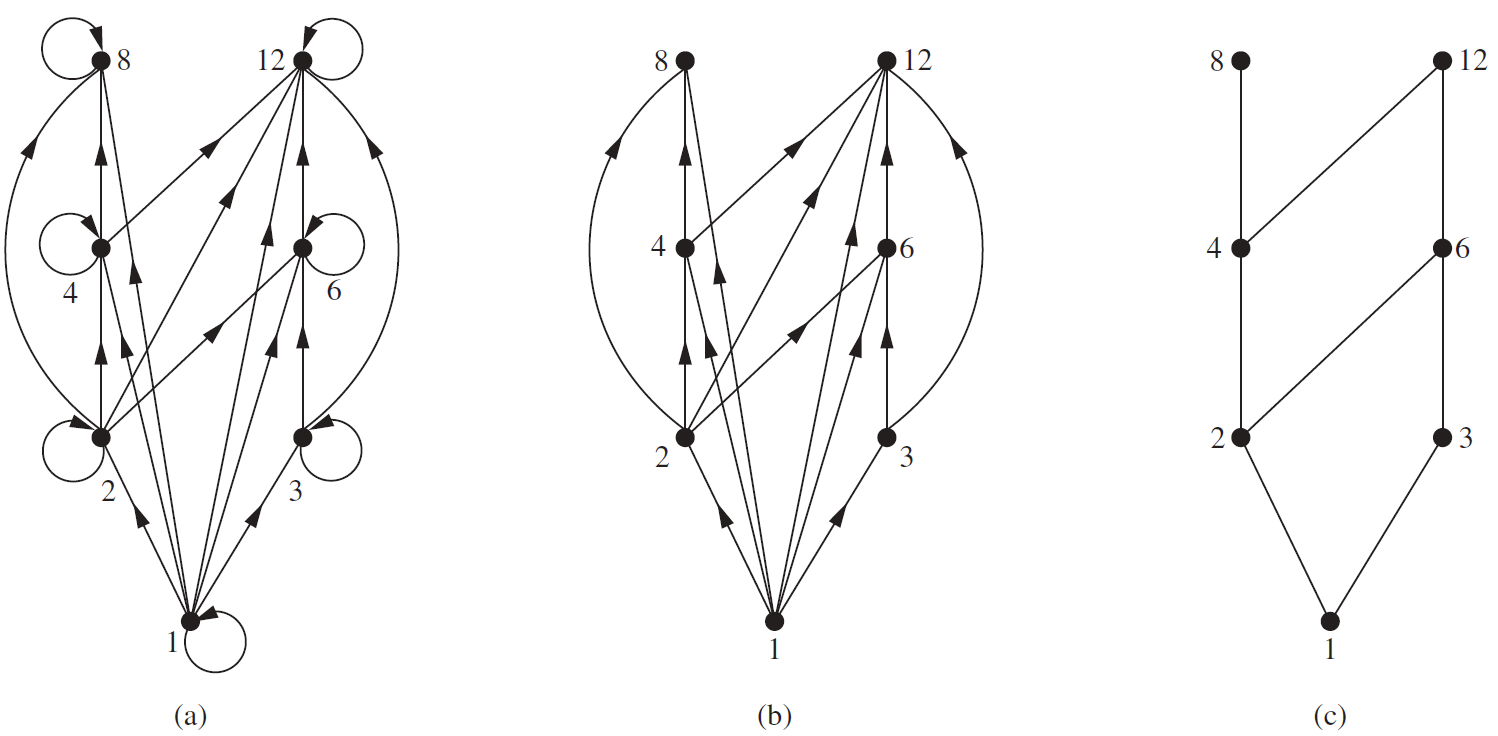
\includegraphics[width=.6\textwidth]{img/ch9.6-f3.png}
    \caption{Constructing the Hasse diagram of (\{1, 2, 3, 4, 6, 8, 12\}, $|$).}
    \label{fig:my_label}
\end{figure}

Let $(S, \preceq)$ be a poset. We say that an element $y \in S$ \textbf{covers} an element $x \in S$ if $x \prec y$ and there is no element $z \in S$ such that $x \prec z \prec y$. The set of pairs $(x, y)$ such that $y$ covers $x$ is called the \textbf{covering relation} of $(S, \preceq)$. From the description of the Hasse diagram of a poset, we see that the edges in the Hasse diagram of $(S, \preceq)$ are upwardly pointing edges corresponding to the pairs in the covering relation of $(S, \preceq)$. Furthermore, we can recover a poset from its covering relation, because it is the reflexive transitive closure of its covering relation.

\subsection{Maximal and Minimal Elements}

\begin{wrapfigure}{r}{0.5\textwidth}
    \centering
    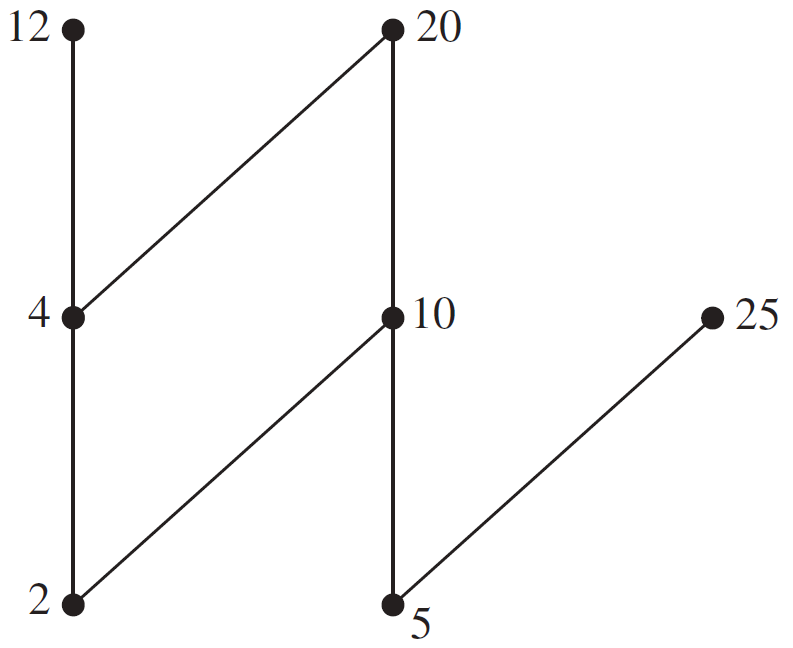
\includegraphics[width=.3\textwidth]{img/ch9.6-f5.png}
    \caption{The Hasse diagram of a poset.}
    \label{fig:my_label}
\end{wrapfigure}

Elements of posets that have certain extremal properties are important for many applications. An element of a poset is called \textbf{maximal} if it is not less than any element of the poset. That is, $a$ is \textbf{maximal} in the poset $(S, \preceq)$ if there is no $b \in S$ such that $a \preceq b$. 

Similarly, an element of a poset is called \textbf{minimal} if it is not greater than any element of the poset. That is, $a$ is \textbf{minimal} if there is no element $b \in S$ such that $b \receq a$. 

\textit{Maximal and minimal elements are easy to spot using a Hasse diagram. They are the “top” and “bottom” elements in the diagram.}

\begin{example}
Which elements of the poset $(\{2, 4, 5, 10, 12, 20, 25\},\ |)$ are maximal, and which are minimal?

\textbf{Solution:}
The Hasse diagram in Figure 5 for this poset shows that the maximal elements are 12, 20, and 25, and the minimal elements are 2 and 5. As this example shows, a poset can have more than one maximal element and more than one minimal element
\end{example}

\begin{wrapfigure}{l}{0.52\textwidth}
    \centering
    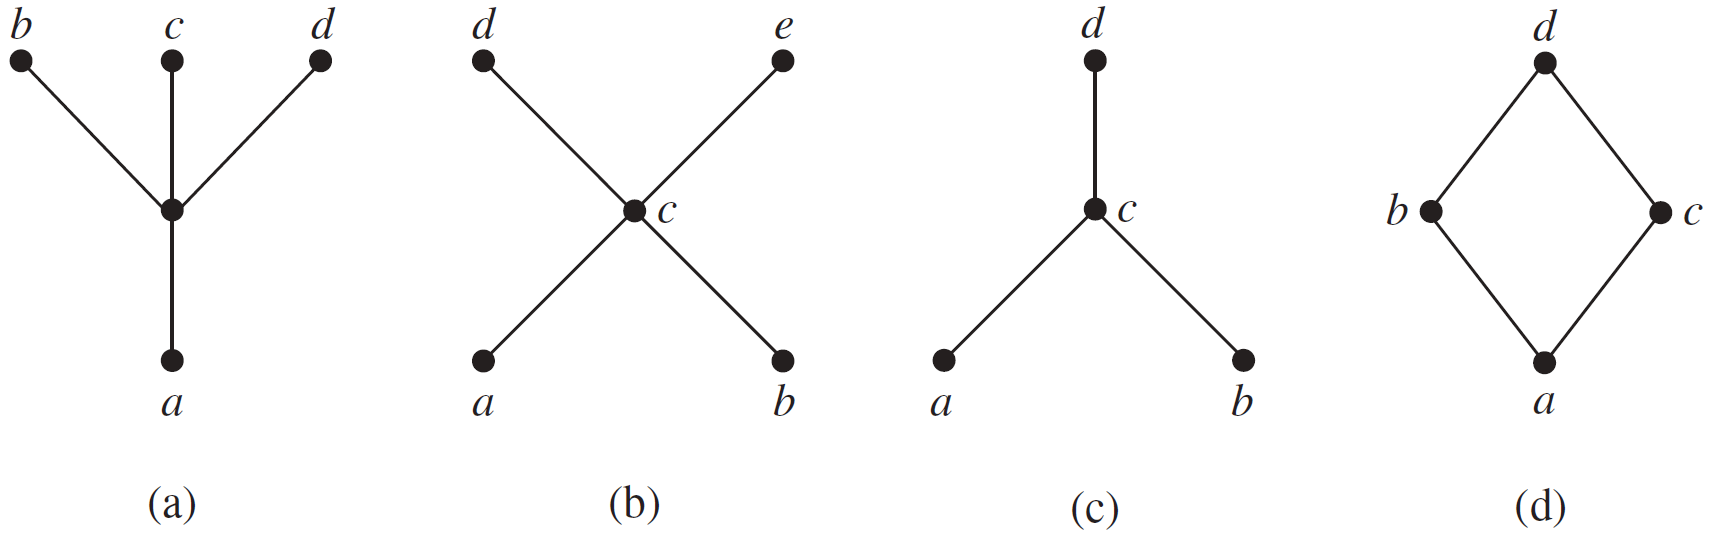
\includegraphics[width=.52\textwidth]{img/ch9.6-f6.png}
    \caption{Hasse diagrams of four posets.}
    \label{fig:my_label}
\end{wrapfigure}

Sometimes there is an element in a poset that is greater than every other element. Such an element is called the \textbf{greatest element}. That is, $a$ is the greatest element of the poset $(S, \preceq)$ if $b \preceq a$ for all $b \in S$. The greatest element is unique when it exists.

Likewise, an element is called the \texbf{least element} if it is less than all the other elements in the poset. That is, $a$ is the least element of $(S, \preceq)$ if $a \preceq b$ for all $b \in S$. The least element is unique when
it exists.


\begin{example}
Determine whether the posets represented by each of the Hasse diagrams in Figure 6 have a greatest element and a least element.

\textbf{Solution:}
The least element of the poset with Hasse diagram $(a)$ is $a$. This poset has no greatest element. The poset with Hasse diagram $(b)$ has neither a least nor a greatest element. The poset with Hasse diagram $(c)$ has no least element. Its greatest element is $d$. The poset with Hasse diagram $(d)$ has least element $a$ and greatest element $d$.
\end{example}

\newpage
Sometimes it is possible to find an element that is greater than or equal to all the elements in a subset $A$ of a poset $(S, \preceq)$. If $u$ is an element of $S$ such that $a \preceq u$ for all elements $a \in A$, then $u$ is called an \textbf{upper bound} of $A$. 

Likewise, there may be an element less than or equal to all the elements in $A$. If $l$ is an element of $S$ such that $l \preceq a$ for all elements $a \in A$, then $l$ is called a lower bound of $A$.

\begin{example}
Find the lower and upper bounds of the subsets $\{a, b, c\}$, $\{j, h\}$, and $\{a, c, d, f\}$ in the poset with the Hasse diagram shown in Figure 7.

\textbf{Solution:}
The upper bounds of $\{a, b, c\}$ are $e$, $f$, $j$, and $h$, and its only lower bound is $a$. There are no upper bounds of $\{j, h\}$, and its lower bounds are $a$, $b$, $c$, $d$, $e$, and $f$. The upper bounds of $\{a, c, d, f \}$ are $f$, $h$, and $j$, and its lower bound is $a$.
\end{example}

\begin{figure}[h!]
    \centering
    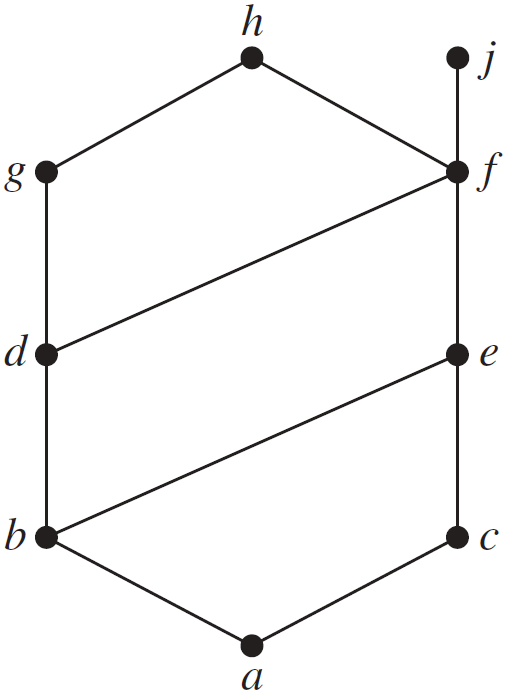
\includegraphics[width=.3\textwidth]{img/ch9.6-f7.png}
    \caption{The Hasse diagram of a poset.}
    \label{fig:my_label}
\end{figure}

The element $x$ is called the \textbf{least upper bound} of the subset $A$ if $x$ is an upper bound that is less than every other upper bound of $A$. Because there is only one such element, if it exists, it makes sense to call this element the least upper bound. That is, $x$ is the least upper bound of $A$ if $a \preceq x$ whenever $a \in A$, and $x \preceq z$ whenever $z$ is an upper bound of $A$.

Similarly, the element $y$ is called the \textbf{greatest lower bound} of $A$ if $y$ is a lower bound of $A$ and $z \preceq y$ whenever $z$ is a lower bound of $A$. The greatest lower bound of $A$ is unique if it exists. 

The greatest lower bound and least upper bound of a subset $A$ are denoted by
$glb(A)$ and $lub(A)$, respectively.

\begin{example}
Find the greatest lower bound and the least upper bound of $\{b, d, g\}$, if they exist, in the poset shown in Figure 7.

\textbf{Solution:}
The upper bounds of $\{b, d, g\}$ are $g$ and $h$. Because $g \preceq h$, $g$ is the least upper bound. The lower bounds of $\{b, d, g\}$ are $a$ and $b$. Because $a \prec b$, $b$ is the greatest lower bound.
\end{example}

\newpage
\subsection{Lattices}

A partially ordered set in which every pair of elements has both a least upper bound and a greatest lower bound is called a \textbf{lattice}. Lattices have many special properties. Furthermore, lattices are used in many different applications such as models of information flow and play an important role in Boolean algebra.

\begin{example}
Determine whether the posets represented by each of the Hasse diagrams in Figure 8 are lattices.

\textbf{Solution:}
The posets represented by the Hasse diagrams in $(a)$ and $(c)$ are both lattices because in each poset every pair of elements has both a least upper bound and a greatest lower bound. 

On the other hand, the poset with the Hasse diagram shown in $(b)$ is not a lattice, because the elements $b$ and $c$ have no least upper bound. To see this, note that each of the elements $d$, $e$, and $f$ is an upper bound, but none of these three elements precedes the other two with respect to the ordering of this poset.
\end{example}

\begin{figure}[h!]
    \centering
    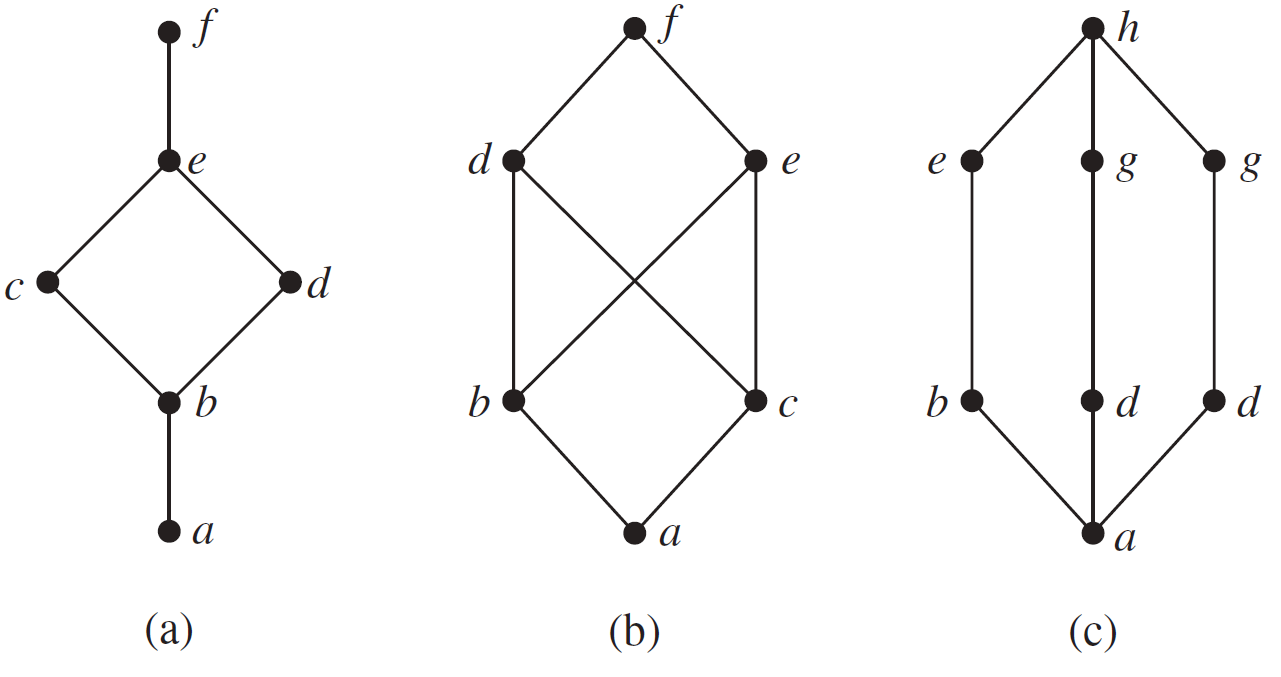
\includegraphics[width=.7\textwidth]{img/ch9.6-f8.png}
    \caption{Hasse diagrams of three posets.}
    \label{fig:my_label}
\end{figure}

\begin{example}
Is the poset $(Z^+, |)$ a lattice?

\textbf{Solution:} Let $a$ and $b$ be two positive integers. The least upper bound and greatest lower bound of these two integers are the least common multiple and the greatest common divisor of these integers, respectively. It follows that this poset is a lattice.
\end{example}

\begin{example}
Determine whether the posets $(\{1, 2, 3, 4, 5\},\ |)$ and $(\{1, 2, 4, 8, 16\}, |)$ are lattices.

\textbf{Solution:}
Because 2 and 3 have no upper bounds in $(\{1, 2, 3, 4, 5\}, |)$, they certainly do not have a least upper bound. Hence, the first poset is not a lattice.

Every two elements of the second poset have both a least upper bound and a greatest lower bound. The least upper bound of two elements in this poset is the larger of the elements and the greatest lower bound of two elements is the smaller of the elements. Hence, this second poset is a lattice.
\end{example}
















\end{document}
